% !Mode:: "TeX:UTF-8"%確保文檔utf-8編碼
%新加入的命令如下:addchtoc addsectoc reduline showendnotes hlabel
%新加入的环境如下:common-format  fig scalefig xverbatim

\documentclass[12pt,oneside]{book}
\newlength{\textpt}
\setlength{\textpt}{12pt}
\newif\ifphone
\phonefalse


\usepackage{myconfig}
\usepackage{mytitle}

\usepackage{wrapfig}

\begin{document}
\frontmatter

\titlea{费曼的}
\titleb{物理学讲义}
\titlec{第一卷}
\author{费曼}
\authorinfo{理查德•费曼(Richard Phillips Feynman,1918年5月11日-1988年2月15日),美国物理学家。1965年诺贝尔物理奖得主。提出了费曼图、费曼规则和重整化的计算方法,这些是研究量子电动力学和粒子物理学的重要工具。}
\editor{德山书生}
\email{a358003542@gmail.com}
\editorinfo{编者:湖南常德人。从网络中找到前五章(不太完整)的txt,感谢这个txt的制作人。}
\version{0.01}
\titleLC

\addchtoc{前言}
\chapter*{前言}
\begin{common-format}
源码在github上。

%这里空一行。

\end{common-format}


\addchtoc{目录}
\setcounter{tocdepth}{2}
\tableofcontents

\begin{common-format}
\mainmatter

\chapter{原子的运动}

\section{引言}
这是一门两学年的物理课,我们开设这门课程是着眼于你们,读者们,将成为物理学工作者。当然,情况并非一定如此,但是每门学科的教授都是这样设想的!假如你打算成为一个物理学工作者,就要学习很多东西;这是一个200年以来空前蓬勃发展的知识领域。事实上,你会想到,这么多的知识是不可能在四年内学完的,确实不可能;你们还得到研究院去继续学习。

相当出人意外的是,尽管在这么长时间中做了极其大量的工作,但却有可能把这一大堆成果大大地加以浓缩。 这就是说,找到一些概括我们所有知识的\uwave{定律}。 不过,即使如此,掌握这些定律也是颇为困难的.。因此在你对科学的这部分与那部分题材之间的关系还没有一个大致的了解之前就让你去钻研这个庞大的课题的话,就不公平了。根据这种看法,前三章将略述物理学与其他科学的关系,各门学科之间的相互联系以及科学的含义,这有助于你们对本学科产生一种切身的感受。

你们可能会问,在讲授欧几里德几何时,先是陈述公理,然后作出各种各样的推论,那为什么在讲授物理学时不能先直截了当地列出基本定律, 然后再就一切可能的情况说明定律的应用呢?(这样一来,如果你不满足于要花四年时间来学习物理,那你是否打算在4分钟内学完它?)我们不能这样做是由于两个理由。 第一,我们还\uwave{不知道}所有的基本定律:未知领域的边界在不断地扩展; 第二,正确地叙述物理定律要涉及到一些非常陌生的概念,而叙述
这些概念又要用到高等数学。因此,即使为了知道\uwave{词}的含义,也需要大量的预备性的训练。的确,那样做是行不通的,我们只能一步一步地来。

大自然整体的每一部分始终只不过是对于整个真理——或者说, \uwave{对于}我们至今所了解的\uwave{整个真理}——的\uwave{逼近}。实际上,人们知道的每件事都只是某种近似,因为\uwave{我们懂得},到目前为止,我们\uwave{确实还不知道所有的定律}。因此,我们之所以需要学习一些东西,正是为了要抛弃以前的谬见,或者更可能的是为了改正以前的谬见。

科学的原则——或者简直可称为科学的定义为:实验是\uwave{一切知识的试金石},实验是科学“真理”的唯一\uwave{鉴定者}。 但是什么是知识的源泉呢?那些要检验的定律又是从何而来的?从某种意义上说,实验为我们提供了种种线索,因此可以说是实验本身促成了这些定律的产生。但是,要从这些线索中作出重大的判断,还需要有丰富的想象力去对蕴藏在所有这些线索后面的令人惊讶、简单、而又非常奇特的图象进行猜测,然后,再用实验来验证我们的猜测究竟对不对。这个想像过程是很艰难的,因此在物理学中有所分工,\uwave{理论}物理学家进行想象、推演和猜测新的定律,但并不做实验;而\uwave{实验}物理学家则进行实验、想象、推演和猜测。

我们说过,自然的定律是近似的:起先我们找到的是“错”的定律,然后才发现“对”的定律。那么,一个实验怎么可能是“错误”的呢?首先,通常是:仪器上有些毛病,而你又没有注意,但是这种问题是容易确定的,可以反复检查。如果不去纠缠在这种次要的问题上,那么实验的结果怎么\uwave{可能}是错误的呢?这只可能是由于不够精确罢了。例如,一个物体的质量似乎是从来不变的,转动的陀螺与静止的陀螺一样重。结果就发现了一条“定律”:质量是个常数,与速率无关。然而现在发现这条“定律”却是不正确的。质量实际上随著速度的加大而增加,但是要速度接近光速,才会显著增加。\uwave{正确}的定律是:如果一个物体的速率小于100海里/秒,那么它的质量的变化不超过百万分之一,在这种近似形式下,这就是一条正确的定律。因此,人们可能认为新的定律实际上并没有什么有意义的差别。当然,这可以说对,也可以说不对。对于一般的速率我们当然可以忘掉它,而用简单的质量守恒定律作为一种很好的近似。但是对于告诉情况这就不正确了:速率越高,就越不正确。

最后,最有趣的是,\uwave{就哲学上而言},使用近似的定律是\uwave{完全错误}的。纵然质量的变化只是一点点,我们的整个世界图景也得改变。这是有关在定律后面的哲学或基本观念的一件十分特殊的事,即使是极小的效应有时在我们的观念上也要引起深刻的变化。

那么,我们应该首先教什么呢?是否应先教那些\uwave{正确}的、陌生的定律以及有关的奇特而困难的观念,例如相对论,四维时空等等之类?还是应先教简单的“质量守恒”定律,即那条虽然只是近似的,但并不包含那种困难的观念的定律?前一条定律比较引人入胜,比较奇特和比较有趣,但是后一条定律在开始时比较容易掌握,它是真正理解前一种观念的第一步。这个问题在物理教学中会一再出现,在不同的时候,我们将要用不同的方式去解决它。但是在每个阶段都值得去弄明白:我们现在所知道的是什么,它的正确性如何,它怎样适应其他的各种事情,以及当我们进一步学习后它会有怎样的变化。

让我们按照我们所理解的当代科学(特别是物理学,但是也包括周围有关的其他科学)的轮廓继续讲下去,这样,当我们以后专门注意某些特殊问题时,就会对于背景情况有所了解——为什么这些特殊问题是有趣的,它们又是怎样适应整体结构的。

那么,我们世界的总体图象是怎样的呢?


\section{物质是原子构成的}
假如由于某种大灾难,所有的科学知识都丢失了,只有一句话传给下一代,那么怎样才能用最少的词汇来表达最多的信息呢\footnote{好问题!}?我相信这句话是原子的假设(或者说原子的事实,无论你愿意怎样称呼都行): 所有的物体都是用原子构成的——这些原子是一些小小的粒子,它们一直不停地运动着。 当彼此略微离开时相互吸引, 当彼此过于挤紧时又互相排斥。只要稍微想一下,你就会发现,在这一句话中包含了大量的有关世界的信息。

为了说明原子观念的重要作用,假设有一滴直径为1/4英寸\footnote{1英寸=2.54厘米,这里指0.635厘米。}的水滴,即使我们非常贴近地观察,也只能见到光滑的、连续的水,而没有任何其他东西并且即使我们用最好的光学显微镜(大致可放大2000倍)把这滴水放大到40英尺\footnote{1英尺=30.40厘米,这里指1216厘米,按照数值是放大了1915倍。}左右(相当于一个大房间那大),然后再靠得相当近地去观察,我们所看到的仍然是比较光滑的水,不过到处有一些足球状的东西在来回游动,非常有趣。这些东西是草履虫。你们可能就到此为止,对草履虫以及它的摆动的纤毛和卷曲的身体感到十分好奇。也许除了把草履虫放得更大一些,看看它的内部外,就不再进一步观察了。当然这是生物学的课题,但是现在我们继续观察下去,再把水放大2000倍更接近地观察水这种物质本身。这时,水滴已放大到有15英里\footnote{1英里=1.609公里,这里指两万四千多米。}那样大了,如果你再十分贴近地观察,你将看到水中充满了某种不再具有光滑外表的东西,而是有些象从远处看过去挤在足球场上的人群。为了能看出挤满的究竟是些什么东西,我们再把它放大250倍后就会看到某种类似于图1-1所示的情形。
\begin{fig}{放大10亿倍的水}
\label{fig:放大10亿倍的水}
\end{fig}
这是放大了10亿倍的水的图象,但是在以下这几方面是理想化了的。首先,各种粒子用简单的方式画成有明显的边缘,这是不精确的。其次,为了简便起见,把它们都画成二维的排列,实际上它们当然是在三维空间中运动的。注意在图中有两类“斑点”或圆,它们各表示氧原子(黑色)和氢原子(白色),而每个氧原子有两个氢原子和它联结在一起(一个氧原子与两个氢原子组成的一个小组称为一个分子)。图象中还有一个被理想化的地方是自然界中的真实粒子总是在不停地跳动,彼此绕来绕去地转着,因而你必须把这幅画面想象成能动的而不是静止的。另一件不能在图上说明的事实是粒子为“粘在一起”的,它们彼此吸引着,这个被那个拉住等等,可以说,整个一群“胶合在一起”,另一方面,这些粒子也不是挤到一块儿,如果你把两个粒子挤得很紧,它们就互相推斥。

原子的半径约为$1\sim2\times10^{-8}$厘米,$ 10^{-8} $厘米现在称为1Å(这只是另一个名称),所以我们说原子的半径为1∼2Å,另一个记住原子大小的方法是这样的:如果把苹果放大到地球那样大,那么苹果中的原子就差不多有原来的苹果那样大。

现在,想象这个大水滴是由所有这些跳动的粒子一个挨一个地“粘合”起来的,水能保持一定的体积而并不散开,因为它的分子彼此吸引。 如果水滴在一个斜面上,它能从一个位置移动到另一个位置。水会流动,但是并不会消失——它们并没有飞逝,因为分子之间有吸引力。这种跳动就是我们所说的热运动,当温度升高时,这种运动就增强了。如果我们加热水滴,跳动就增加,原子之间的空隙也增大。如果继续加热到分子间的引力不足以将彼此拉住时,它们就分开来飞散了。当然,这正是我们从水制取水蒸气的方法——提高温度,粒子由于运动的增强而飞散。图 1-2是一幅水蒸气的图象。
\begin{fig}{水蒸气}
\label{fig:水蒸气}
\end{fig}
这张水蒸气图象有一个不足之处:在通常的气压下在整个房间里只有少数几个分子,决不可能在这样一张图象中有三个以上的分子。在大多数情况下,这样大小的方块中可能连一个都不会有——不过碰巧在这张图中有两个半或三个分子(只有这样图象才不会是完全空白的)。现在比起水来,在水蒸气的情况下,我们可以更清楚地看到水所特有的分子。为了简单起见,将分子画成具有120°的夹角,实际上,这个角是105°3′,氢原子中心与氧原子中心之间的距离是0.957Å。这样看来,我们对这个分子了解得很清楚了。

让我们来看一下,水蒸气或任何其他气体具有一些什么性质。这些气体分子是彼此分离的,它们打在墙上时,会反弹回来。设想在一个房间里有一些网球(100个左右)不断地来回跳动,当它们打到墙上后,就将墙推离原位(当然,我们必须将墙推回去)。这意味着气体施加一个“颤动”的力,而我们的粗糙的感官(并没有被我们自己放大十亿倍)只感到一个平均的推力。为了把气体限制在一定的范围之内,我们必须施加一个压力。图1-3是一个盛气体的标准容器(所有教科书中都有这种图)
\begin{fig}{一个配有活塞的汽缸}
\label{fig:一个配有活塞的汽缸}
\end{fig}
一个配有活塞的汽缸,由于不论水分子的形状如何,情况都是一样,因此为简单起见,我们把它们画成网球形状或者小黑点。这些东西沿着所有的方向不停地运动着。由于有这么多的气体分子一直在撞击顶端的活塞,因此要使活塞不被这种不断的碰撞逐渐顶出来必须施加一定的力把活塞压下去,这个力称为\uwave{压力}(实际上,是压强乘以面积)。很清楚,这个力正比于面积,因为如果我们增大面积而保持每立方厘米内的分子数不变的话,那么分子与活塞碰撞次数增加的比例与面积增加的比例是相同的。

现在让我们在这个容器内放入两倍的分子,以使密度增加一倍,同时让它们具有同样的速度,即相同的温度。那么,作为一种很好的近似,碰撞的次数也将增加一倍,由于每次碰撞仍然和先前那样“有力”,压力就正比于密度。如果我们考虑到原子之间的力的真实性质,那么由于原子之间的吸引,可以预期压力略有减少;而由于原子也占有有限的体积,则可以预期压力略有增加。无论如何,作为一个很好的近似,如果原子较少,密度足够低,那么,\uwave{压力正比于密度}。

我们还可以看一下其他情况。如果提高温度而不改变气体密度,亦即只增加原子的速度,那么在压力上会出现什么情况?当然,原子将撞击得更剧烈一些,因为它们运动得更快一些。此外,它们的碰撞更频繁了,因此压力将增加,你们看,原子理论的概念是多么简单!

我们来考虑另一种情况,假定活塞向下移动,原子就慢慢地被压缩在一个较小的空间里。当原子碰到运动着的活塞时,会发生什么情况呢?很显然,原子由于碰撞而提高了速率,例如,你可以试一下乒乓球从一个朝前运动的球拍弹回来时的情况,你会发现弹回的速率比打到球拍上的速率更大一些(一个特例是如果一个原子恰好静止不动,那么在活塞碰上它以后,当然就运动了)。这样原子在弹离活寒时比碰上去之前更“热”因此所有容器中的分子的速率都提高了。这意味着,\uwave{当我们缓慢压缩气体时,气体的温度会升高}。结果,在缓慢压缩时,气体的温度将升高;而在缓慢膨胀时,气体的温度将降低。

现在回到我们的那滴水上去,从另一个角度去观察一下,假定现在降低水滴的温度,并且假定水的原子、分子的跳动逐渐减小。我们知道在原子之间存在着引力,因而过一会儿,它们就不能再跳得那么厉害了。图1-4表示在很低的温度下会出现什么样的情况。这时分子连接成一种新的图象,这就是冰。
\begin{fig}{冰}
\label{fig:冰}
\end{fig}
这个特殊的冰的图象是不正确的,因为它只是二维的,但是它在定性上是正确的。有趣的一点是,\uwave{对于每一个原子,都有它的确定位置}。你们可以很容易地设想,如果我们用某种方式使冰的一端的所有的原子按一定的方式排列,并让每个原子处在一定的位置上,那么由于互相连接的结构很牢固,几英里之外(在我们放大的比例下)的另一端也将有确定的位置。如果我们抓住一根冰棍的一端,另一端就会阻止我们把它拉出去。这种情况不象水那样由于跳动加强以致所有的原子以种种方式到处跑来跑去, 因而结构也就
被破坏了。固体与液体的差别就在于:在固体中,原子以某种称为\uwave{晶体排列}的方式排列着,即使在较长的距离上它们的位置也不能杂乱无章。晶体一端的原子位置取决于晶体另一端的与之相距千百万个原子的排列位置。图1-4是一种虚构的冰的排列状况,它虽然包括了冰的许多正确的特征,但并不是真实的排列情况。正确的特征之一是这里具有一种六边形的对称性。你们可以看到:如果把画面绕一根轴转动120°的话,它仍然回到原来的形状,因此,在
冰里存在着一定的对称性,这说明为什么雪花具有六边形的外表。从图1-4中还可以看到为什么冰融解时会缩小。在这里列出的冰的晶体图样中有许多“孔”,真实的冰的结构也是如此,在排列打散后,这些孔就可以容纳分子。除水和铅字合金\footnote{铅、锑、锡的合金,也称为活字合金。}外,许多简单的物质在融解时都要膨胀,因为在固体的晶体结构中,原子是密集堆积的,而当熔解时,需要有更多的空间供原子活动,但是敞形结构则会倒坍,体积反而收缩了,就象水的情况那样。

虽然冰有一种“刚性的”结晶形态,它的温度也会变化——冰也储存热量,如果我们愿意的话,就可以改变热量的储存。对冰来说,这种热量指的是什么呢?冰的原子并不是静止不动的,它们不断地摇晃着、振动着,所以虽然晶体存在着一种确定的次序——一种确定的结构,所有的原子仍都“在适当的位置”上振动,当我们提高温度时,它们振动的幅度就越来越大,直到离开原来的位置为止。我们把这个过程称为熔解,当降低温度时,振动的幅度越来越小,直到绝对零度原子仍能有最低限度的振动,而\uwave{不是停止}振动。原子所具有的这种最低的振动不足以使物质熔解,只有一个例外,即氦。在温度降低时,氦原子的运动只是尽可能地减弱,但即使在绝对零度时也有足够的运动使之不致于凝固,除非把压力加得这样大以致将原子都挤在一起。如果我们提高压力,就可以使它凝固。


\section{原子过程}
关于从原子的观点来描写固体、液体和气体,我们就讲到这里。然而原子的假设也可以描写\uwave{过程},所以我们现在从原子的观点来考察一些过程。我们要考察的第一个过程与水的表面有关。在水的表面有些什么情况呢?设想水的表面上是空气,现在我们来把图画得更复杂一些——也更实际一些,如图1-5所示。
\begin{fig}{空气中水的蒸发}
\label{fig:空气中水的蒸发}
\end{fig}
我们看到,水分子仍然象先前那样,组成大量的水,但现在还看到水的表面。在水面上我们发现一些东西:首先,水面上有水的分子,这就是\uwave{水的蒸气},在水面上总是有水蒸气的。(在水蒸气与水之间存在着一种平衡,这种平衡我们以后再讲。)此外,我们还发现一些别的分子:这里是两个氧原子彼此结合在一起组成一个\uwave{氧分子},那里是两个氮原子结合在一起组成一个氮分子。空气几乎完全是由氮气、氧气、水蒸气组成的,此外还有少量的二氧化碳、氩气和其他一些气体。所以在水面上的是含有一些水蒸气的气体。那么在这种情况下会发生什么事呢?水里的分子不断地晃来晃去。有时,在水面上有个别分子碰巧受到比通常情况下更大的冲击而被“踢”出表面。因为图1-5是\uwave{静止}的画面,所以在图上难以看出所发生的事。但是我们可以想象表面附近的某一个分子刚好受到碰撞而飞了出去,或者也许另一个分子也受到碰撞而飞了出去。分子一个接着一个地跑了出去,水就消失了——蒸发了。但是如果把容器盖上,过了一会儿就会发现在空气分子中有大量的水分子。水蒸气的分子不时地飞到水面,又回到水中。结果,我们看到那个看来死气沉沉的、无趣的事情——杯盖上的可能已放了二十年的水——实在包含了一直生气勃勃而有趣的现象。对我们这双肉眼而言,看不出有任何变化,但是如果能放大十亿倍来看的话,我们就能发现情况一直在变化,一些分子离开水面,又一些分子则回到了水面。

为什么\uwave{我们看不出变化呢}?因为有多少分子离开水面就会有多少分子回到水面!归根到底“没有任何事情发生”如果现在我们把容器盖打开,使潮湿的空气吹走而代之以干燥空气,那么离开水面的分子数还是如先前那样多,因为这只取决于水分子晃动的程度,但是回到水面的分子数则大大地减少了,因为在水面上的水分子数已极其稀少。因此逸出水面的分子比进入水面的分子多,水就蒸发了。所以,如果你要使水蒸发的话,就打开风扇吧!

这里还有另一件事情:哪些分子会离开?一个分子能离开水面是由于它偶然比通常情况稍微多积累了一些能量,这样才能使它摆脱邻近分子的吸引。结果,由于离开水面的分子带走的能量比平均能量大,留在水中的分子的运动平均起来就比先前\uwave{减弱}。因此液体蒸发时会逐渐冷却。当然,当一个水蒸气分子从空气中跑向水面时,它一靠近水面就要突然受到一个很强的吸引。这就使它进入水中时具有更大的速度,结果就产生热量。所以当水分子离开水面时,它们带走了热量;而当它们回到水面时, 则产生了热量。当然,如果不存在净的蒸发现象的话,什么结果也不会发生——水的温度并不改变。如果我们向水面上吹风,使蒸发的分子数一直占优势,水就会冷却。因此,要使汤冷却就得不停地吹\footnote{这里翻译“当然”说得太多了,作者就喝汤说事,幽默于胸啊。}!

当然,你们应当了解,刚才所说的那个过程实际上要比我们所指出的更为复杂。不仅水分子进入空气,不时还有氧分子或氮分子跑到水里,“消失”在一大堆水分子中,这样空气就溶解在水中了。氧和氮的分子进入水中,水里就含有空气。如果我们突然从容器中抽走空气,那么空气分子出来要比进去来得快,这样就形成了气泡。你们可能知道,这对潜水员是很不利的\footnote{所谓的减压病}。

现在我们来考虑另一种过程。在图1-6中,我们从原子的观点来看固体在水中溶解。
\begin{fig}{盐在水中的溶解}
\label{fig:盐在水中的溶解}
\end{fig}
如果我们把结晶盐粒丢入水中,会出现什么情况呢?食盐是一种固体,也是一种晶体,并且是“食盐原子”的有规则的排列。
\endnote{严格意义上讲任何物质在固态都会达到一种热力学自由能最低时候的状态,这个时候的固体就是晶体。只是有些物质在相当长的时间内都不能形成晶体,他们通常被称之为粘稠的液体或者凝固了的液体。比如塑料,橡胶,玻璃,蜡烛等。像这些物质都没有确定的熔点。}
图1-7是普通食盐——氯化钠的三维结构图。
\begin{fig}{食盐的晶体结构}
\label{fig:食盐的晶体结构}
\end{fig}
严格地说, 这种晶体不是用原子而是用我们所谓的\uwave{离子}构成的!离子就是带有额外电子的原子,或失去一些电子的原子。在食盐晶体中我们发现了氯离子(带有一个额外电子的氯原子)和钠离子(失去一个电子的钠原子)。在固态食盐中,所有的离子都由于电的作用而吸引在一起,但是当我们把食盐投到水里后,就会发现,所有的离子都由于电的作用而吸引在一起,有一些离子离散了。在图1-6中有一个氯离子松开来了,其他的原子则以离子的形式在水中浮动。这张图画得相当仔细:例如,注意水分子中的氢原子一端大多靠近氯离子,而在钠离子周围所见到的大多是氧原子的那一端,因为钠是正的,而水的氧原子一端是负的,它们之间有电的吸引。我们能不能从这幅图画中看出盐究竟是\uwave{溶解于}水中,还是从水中\uwave{结晶出来}?当然,我们看不出来,因为当某些原子离开晶体时,另一些原子又重新聚集到晶体上。整个过程是一个\uwave{动态过程},犹如同蒸发的情况,它取决于水中盐的含量是超过还是少于形成平衡所需要的数量。所谓平衡我们指的是这种情况,即原子离开晶体的比率正好与回到晶体的比率相同。假如在水中几乎没有什么盐,离开的原子就比回去的原子多,食盐就溶解。但另一方面,如果水里的“食盐原子”太多,那么回去的就多于离开的,食盐就结晶。

我们顺便说一下,物质的分子这个概念只是近似的,而且只是对某些种类的物质才有意义。很清楚,在水的情况下,三个原子彼此确实站在一起。但是在固体的氯化钠情况下就不那么明确了。在氯化钠中钠离子和氯离子只是以立方体的形式排列。这里没有一种把它们自然分成“食盐分子”的方式。

现在回到我们的溶解与淀积\footnote{沉淀并积聚}的讨论上。如果增加食盐溶液的温度,那么原子离开的比率就会增加,而原子回来的比率也会增加。结果是一般很难预言会朝哪一个方向发展,固体
溶解得多一些还是少一些。当温度提高时,大多数物质更易溶解, 但是某些物质则更不易溶解。

\section{化学反应}
到现在为止,在我们所描述的一切过程中,原子和离子的伙伴并没有变更,但是当然也有这种情况,原子的组合的确改变了,形成新的分子。图1-8就是说明这一情况的。在一个过程中如果原子的伙伴重新排列,我们就称之为\uwave{化学反应}。其他前面所描述的过程称为物理过程,但是二者之间并没有明显的界限(大自然并不关心我们究竟如何去称呼,她只知道不断地进行工作)。图1-8表示碳在氧气中的燃烧。
\begin{fig}{碳在氧气中的燃烧}
\label{fig:碳在氧气中的燃烧}
\end{fig}
在氧气中,\uwave{两个}氧原子紧紧地吸引在一起(为什么不是\uwave{三个}甚至四个吸引在一起?这是此类原子过程的一个很典型的特征。原子是非常特别的:它们喜欢一定的伙伴,一定的方向,等等。物理学的任务就是要分析每一个原子为什么想要它所希望要的东西。无论如何,两个氧原子形成了一个饱和的、适宜的分子。)

这些碳原子应该处于固态晶体之中(可以是石墨,也可以是金刚石\footnote{金刚石在空气中也可以燃烧}。)现在,比如说有一个氧分子跑到碳这边来,每个氧原子可以抓住一个碳原子而以一种新的组合——“碳-氧”——一起飞走,这就是所谓的一氧化碳气体分子,它的化学名称是CO。这种气体分子很简单:字母“CO”实际上就是这个分子的一个画象。但是碳吸引氧的能力比氧吸引氧或者碳吸引碳的能力更大。因此在这个过程中氧原子可能在到达时只带有一点点能量,但是氧和碳的结合却是非常彻底而剧烈的,所有靠近它们的原子都吸收能量。于是就产生了大量的分子运动的能量——动能。当然,这就是燃烧。我们从氧和碳的结合得到了\uwave{热量}。这种热量通常是以热气体的分子运动的形式存在的,但是在某些情况下,由于热量非常大而\uwave{发出了光}。这就是怎样产生火焰的过程。

此外,一氧化碳分子并不感到满足。它可能再缚住另一个氧原子,因此可能出现远为复杂的反应:氧与碳会结合起来,同时偶尔又与一氧化碳分子碰撞。于是一个氧原子可能结合到一个CO分子上,最终形成另一个分子,它包含一个碳原子和两个氧原子,称为二氧化碳,并以\chemfig{CO_2}表示。假如我们以很快的速度在很少的氧气中燃烧碳的话(例如,在汽车引擎中,爆炸是如此迅速,以致没有时间形成二氧化碳),就形成了大量的一氧化碳。在许多这种重新排列的过程中,大量的能量被释放出来,依反应条件的不同而形成爆炸、火焰等等。化学家研究了这些原子的排列情况,发现每一种物质都是某种类型的\uwave{原子的排列}。

为了说明这个概念,我们来考虑另一个例子。如果我们走到一个紫罗兰花圃里去,我们知道那是一种什么香气。这是某种\uwave{分子}或者说原子排列钻进了我们的鼻子。首先,这种分子是怎样钻进来的呢?这很容易。假如香气是飘浮在空气中的某种分子,它们就会到处晃动,四面八方地撞来撞去,很可能偶尔钻进了我们的鼻子。肯定分子并不想特别进入我们的嗅觉器官。在挤成一堆的分子中,大家都无目的地到处徘徊,而碰巧有一些分子却发现自己原来已到达人的鼻子中了

现在,化学家可以取一些象紫罗兰香气这样特殊的分子进行分析,然后告诉我们原子在空间的\uwave{精确排列}。我们知道二氧化碳分子的结构是简单而对称的:\chemfig{O=C=O}。(这也很容易用物理方法来确定。)然而,即使对化学中那些非常复杂的原子队列,人们也可以通过长期的、卓越的探索工作来查明其排列方式。图1-9是空气中紫罗兰香气图。
\begin{fig}{空气中的紫罗兰香气分子}
\label{fig:空气中的紫罗兰香气分子}
\end{fig}
我们再一次发现有氮、氧以及水蒸气。(为什么这儿有水蒸气?因为紫罗兰是湿的。所有的植物都会蒸发水气。)然而,我们还看到一个由碳原子、氧原子及氢原子组成的“怪物”,它也选择了一种特殊的排列形式。这种形式比二氧化碳的排列远为复杂;事实上,它是一种极为复杂的排列。遗憾的是,我们无法画出所有那些在化学上已确实知道的情况,因为所有的原子的精确排列都是三维的,而我们的画面只是二维的。六个碳原子组成了一个环,但它不是扁平的,而是一种“皱褶”的环。环的所有角度和间距都已知道。所以一个化学式只是这样的分子的一个画象。当一位化学家把它写在黑板上时,粗略地说,他是在二维空间里“画”图。比如,我们见到六个碳原子组成的一个“环”,在一个端点还悬挂着一条碳“链”,链的第二个端点的碳上有一个氧原子,还有三个氢原子连在那个碳原子上,两个氢原子和三个碳原子竖在这儿,等等。

化学家是怎样发现这种排列的呢?他把几瓶东西混合起来,如果变红了,就说明,在某处有两个碳原子与一个氧原子联结在一起;如果变蓝了,就说明根本不是那么一回事。这是所做过的最奇妙的探索工作之一——有机化学。为了发现极其复杂的阵列中的原子排列,化学家观察两种不同的物质混合后究竟会发生什么事?当化学家描述原子的排列时,物理学家从来不怎么相信化学家了解他在谈论的是什么。大约在20年前就能在某些情况下用物理方法来研究这些分子的排列(不完全象我们这个分子那样复杂,只包括了它的一部分),而且能通过\uwave{测量}而不是观察颜色来确定每个原子的位置,嗨!你瞧!化学家几乎总是正确的。

结果,实际上紫罗兰的香气里有三种略为不同的分子,其差别仅在于氢原子的排列不同。

化学的一个任务是给物质命名,从而使我们知道它是什么。给这种形状起个名字看看,这个名称不仅要表明形状,而且还要说出这里是一个氧原子,那里是一个氢原子——确切地说出每 个原子的名称和位置。所以我们可以设想,为了全面起见,化学名称一定是十分复杂的。你们看!这个东西的比较完整的名称是4(2, 2, 3, 6-四甲基-5-环己烯基)-3-丁烯-2-酮,它告诉你这样东西的结构,还告诉你这就是它的排列方式。我们可以意识到化学家所遇到的困难,也懂得这样长的命名的理由。化学家们并不想把名称搞得这样晦涩难懂,但在试图用词汇来描写分子时,他们却遇到了非常棘手的问题!

图1-10是α鸢尾酮香料的分子结构图。
\begin{fig}{α鸢尾酮香料的分子结构图}
\label{fig:α鸢尾酮香料的分子结构图}
\end{fig}

我们怎么\uwave{知道}存在着原子呢?可以用上面提到过的一种技巧:我们\uwave{假设}存在着原子,而一个又一个的结果与我们的预言相符合,如果事物真\uwave{是}由原子组成的话,它们就应当如此。此外,也多少有点更为直接的证据,下面就是一个很好的例子。由于原子是如此之小,你用光学显微镜观察不到它,事实上,即使用\uwave{电子}显微镜也不行。(用光学显微镜,你们只能看到大得多的的东西。)要是原子一直在运动,比如水中的原子,那么如果我们把某种较大的球放到水中去,这个比原子大得多的球就会晃来晃去——就像玩球时,一个很大的球被许多人打来打去一样。人们向各个方向推球,结果球在场地上作不规则运动。同样,“大球”也将运动,因为它在各个方面受到的碰撞不等,在各个时刻受到的碰撞也不等。因此,如果我们用很好的显微镜观察水中很小的粒子(胶粒),就能看到微粒在不停地跳动,这是原子碰撞的结果。这种运动称为\uwave{布朗运动}。

我们在晶体结构上也可看到进一步的证据。在许多情况下,由X射线分析推断出的结构在空间“形状”上与自然界中的晶体实际上显示出来的形状相符合。实际晶体的各个“面”之间的夹角,与从晶体是由多“层”原子构成的假设推断出来的角度之差在秒以下。

\uwave{一切都由原子构成}。这就是关键性的假设。例如,在整个生物学中最重要的假设是:\uwave{动物所作的每件事都是原子做的}。换句话说:\uwave{没有一件生物做的事情不能从这些生物是用服从物理定律的运动原子组成的这个观点来加以理解}。这在开始并没有认识到:提出这种假设需要做一些实验与推理,但现在它已被接受了,它是在生物学领域内产生新观念的最有用的理论。

如果一块由一个挨一个的原子组成的钢或盐可以具有这种有趣的性质:如果水——它只不过是些小滴,地球上到处都有——可以形成波浪和泡沫,那这些波浪冲向水泥堤岸时会产生冲击声和奇妙的浪花;如果一流溪水永远只能是一堆原子,那么还会有什么呢?假设我们不是把原子排成确定的形式,再三重复,不断反复,或者甚至形成向紫罗兰香气那样复杂的东西,那么事情会变得更加不可思议吗?——那个在你面前走来走去与你攀谈的东西可能是一大群排列的非常复杂的原子吗?这个东西的彻底复杂性可能动摇你对它产生一些什么想象吗?当我们说,我们是一堆原子,这并不意味着我们\uwave{只是}一堆原子,当你站在镜子前,你就能在镜子里看到,一堆并非简单地一个一个重复排列的原子所组成的东西将会具有如何丰富和生动的内容!


\section{注释}
\showendnotes




\chapter{基本物理}
\section{引言}
在本章中,我们将考察有关物理学的最基本概念——即我们在目前所知道的事物的本性。这里将不去涉及我们如何知道所有这些观念是正确的那个认识过程,你们在适当的时候会学习到这些具体的细节。

我们在科学上所关心的事物,具有无数形式和许多属性。举例来说,假如我们站在岸边眺望大海,将会看到:这里有海水、拍击的浪花、飞溅的泡沫以及汹涌的波浪,还有太阳、光线、蔚蓝的天空、白云以及空气的流动——风;在海边有沙粒,不同色纹和硬度的岩石;在海里浮游着生物,此生彼灭;最后,还有我们这些站在海岸边的观察者;甚至还有幸福和怀念。在自然界的其他场合,难道不也同样出现如此纷繁复杂的事物和影响吗?无论在哪里,到处都是这样错综复杂和变化无穷。好奇心驱使我们提出问题,把事物联系起来,而将它们的种种表现理解为:或许是由较少量的基本事物和相互作用以无穷多的方式组合后所产生的结果。

例如,沙粒和岩石是两回事吗?就是说,沙粒只不过是大量的细小石块吗?月亮是不是一块巨大的岩石呢?如果我们了解岩石,是否就能了解沙粒和月亮呢?风是否与海洋中的水流相似,就是一种空气的流动?不同的运动有什么共同特征?不同的声音有什么相似之处?究竟有多少种颜色?等等,等等。我们就是试图这样地逐步分析所有的事情,把那些乍看起来似乎不相同的东西联系起来,希望有可能\uwave{减少不同类}事物的数目,从而能更好的理解它们。

几个世纪以前,人们想出了一种部分解答这类问题的方法,那就是:\uwave{观察},\uwave{推理}和\uwave{实验};这些内容构成了通常所说的\uwave{科学方法}。在这里,我们将只限于对那些有时称之为基本物理中的基本观点,或者由于应用科学方法而形成的基本概念作一描述。

现在我们要问:所谓“理解”某种事情指的是什么意思?可以作一想象:组成这个“世界”的运动物体的复杂排列似乎有点像是天神们所下的一盘伟大的象棋(这里指的是国际象棋——译者注),我们则是这盘棋的观众。我们不知道弈棋的规则,所有能做的事情就是\uwave{观看}这场棋赛。当然,假如我们观看了足够长的时间,总归能看出几条规则来,这些弈棋规则就是我们所说的基本物理。但是,即使我们知道了每条规则,仍然有可能不理解为什么下棋时要走某一步棋,这仅仅是因为情况太复杂了,而我们的智力却是有限的。如果你们会下棋,就一定知道,学会所有的规则是容易的,但是,要选择最好的一着棋,或者要弄懂别人为什么走这一着棋,往往就很困难了。在自然界里,也正是如此,而且只有更难一些。但是,至少我们能发现所有的规则。实际上我们今天还没找到一切规则(时而会出现一些像弈棋中“以车护王”那样的情况,使我们仍然感到无法理解)。除此之外,我们确实能用已知规则来解释的事情也是非常有限的,因为几乎所有的情况都是极其复杂的,我们不能领会这盘棋中应用这些规则的走法,更无法预言下一步将要怎样。所以,我们必须使自己只限于弈棋规则这个比较基本的问题。如果我们知道了规则,就认为“理解”了世界。

如果我们不能很好的分析这盘象棋游戏,那么又怎样来辨别我们“猜测”出的规则实际上是否正确呢?大致地讲,可以有三种办法。第一,可能有这种情况:大自然安排的,或者说我们将大自然安排的十分简单,只有少数几个组成部分,从而使我们能够正确地预测将要发生的事。在这种情况下,就能检验我们的规则是怎样起作用的。(在棋盘角落里可能只有少数几个棋子在移动,所以我们能够正确地解决。)

第二种检验规则的好办法是,利用那些由已知规则推导出来的一些较一般性的法则来检验已知规则本身。比如,象在棋盘中移动的规则是只许走对角线,因而我们可以推断,无论象走了多少步,它总是出现在红方块里。这样,即使不能领会细节,我们也总能检验有关象的走法的概念,只要弄清楚它是否一直在红方块里。当然,在相当长的时间里,它都将如此,直到突然发现它出现在黑方块里。(显然,这时发生的情况是这个象被俘获了,另一个卒走过来成为皇后,红方块里的象就变成黑方块里的象。)这也就是物理学中出现的情况,即使我们不能领会其中的细节,但是在相当长的时期内我们仍有在各方面都很好地起作用的规则;但是在某个时候,我们又会发现新的规则。从基本物理的观点来看,最有趣的现象当然是在那些\uwave{新的}场合——那些已知规则行不通的场合中所出现的现象,而不是在原有规则行得通的地方发生的现象!这是我们发现新规则的一条途径。

第三个鉴别我们的观念是否正确的方法比较粗糙,但或许是所有方法中最为有效的。这就是用粗略的近似方法来加以辨别。我们可能说不出为什么阿莱克因(Alekhine)\footnote{世界著名弈棋手,系国际象棋大师。曾多次获得国际象棋世界冠军。——译者注}要走这步棋,但是我们或许能大致认为它或多或少地在调集一些棋子到王的周围来保护它。因为这是在这种情况下明摆着的事。同样,根据我们对这盘棋的理解,即使不能看出每一步棋的作用,也常常能对自然界多少有所理解。

人们首先把自然界中的现象大致分为几类,如热、电、力学、磁、物性、化学、光或光学、X射线、核物理、引力、介子等等现象。然而,这样做的目的,是将\uwave{整个自然界}看作是一系列现象的许多不同侧面。这就是今天基础理论物理面临的问题:\uwave{发现隐匿在实验后的定律};\uwave{把各类现象综合起来}。在历史上,人们总能做到这一点,但随着时间的推移,新的事实发现了;我们曾经将现象综合得很好,突然,发现了 X 射线,随后我们又融合了更多事实,但是又发现了介子。因此,在弈棋的任何一个阶段,看起来总是相当凌乱。大量事实被归并了,但总还有许多线索向一切方向延伸出去。这就是今天的状况,也就是我们将试图去描绘的现状。

历史上出现过的若干进行综合的情况有如下几个。首先,是\uwave{热}与\uwave{力学}的综合,当原子运动时,运动得越是剧烈,系统所包含的热量就越多,这样,\uwave{热和所有的温度效应}可以用力学定律来说明。另一个巨大的综合,是发现了电、磁、光之间的联系,从而知道它们是同一件事物的不同方面,即今天我们称为\uwave{电磁场}的那个东西的不同表现。还有一个综合,是把化学现象、各种物质的各种性质以及原子的行为统一起来,这就是\uwave{量子化学}的内容。

显然,现在的问题是:能不能继续把所有的事情都综合起来,并且仅仅发现这整个世界体现了\uwave{一件}事情的种种不同方面?无人知道答案如何,我们所知道的只是:这样做下去时,我们发现可以综合一些事实,随后又发觉出现了一些不能综合的事实。我们继续尝试这种拼图游戏。至于是否只有有限数量的棋子,甚至这场拼图游戏是否有底,当然不知道。除非有那么一天终于把拼图拼成了,否则我们就永远不会知道事情的究竟。在这里我们要做的是,看看那种综合已经到了什么程度,在借助于最少的一组原理来理解基本现象方面,现状又是如何。简言之,\uwave{事物是用什么构成的}?\uwave{总共存在多少基本元素}?

\section{1920年以前的物理学}
一开始就从现在的观点讲起是有点困难的,所以让我们先来看一下在1920年左右人们是怎样看待世界的,然后再从这幅图像中挑出几件事情来。在1920年以前,我们的世界图像大致是这样的:宇宙活动的“舞台”是欧几里德所描绘的三维几何\uwave{空间},一切事物在称为\uwave{时间}的某一种媒质里变化,舞台上的基本元素是\uwave{粒子},例如原子,它们具有某些\uwave{特性},首先一个特性是惯性:如果一个粒子正在运动,那么它将沿着同一个方向继续运动下去,除非有\uwave{力}作用其上。此外,第二个基本元素就是\uwave{力},当时认为共有两类力。第一类力是一种极其复杂细致的相互作用,它们以复杂的方式将各种各样的原子约束在不同的组合之中,它们确定当温度升高时,食盐是溶解的更快还是更慢些;另一类已知的力是一种长程的相互作用,它是与距离平方成反比的变化平缓的作用力,称为万有引力。这条定律已为我们所知,它是很简单的。当然,\uwave{为什么}物体的运动一经开始就能保持下去,或者说\uwave{为什么}存在一条万有引力定律,我们则不清楚。

对自然的描述正是我们在这里要关心的。从这个观点出发,气体以及实际上\uwave{所有}的物质都是无数运动着的原子。这样,我们站在海边所听见到的许多东西马上可以联系起来了。首先是压力,它是来自原子与墙或者某个东西的碰撞;如果原子的运动平均而言都是沿着一个方向,这种原子的漂移运动就是风;而无规则的内部运动就是热。某个地方有过多的原子集结在一起时,就形成了过剩密度的波,当波前进时,把成堆的原子推向更远的地方,等等。这种过剩密度的波就是声波。能够理解这么多事情的确是惊人的成就。在前一章里,我们已经说明过一些这样的事情。

粒子有哪些种类?在当时认为有 92 种:那时已经发现有 92 种不同的原子,各按其化学性质而被赋予不同的名称。

其次的问题是“短程力”是什么?为什么碳吸引一个(有时两个)而不是三个氧?原子间的相互作用的机制是什么?是万有引力吗?答案是否定的。万有引力实在是太弱了。于是让我们来设想一种类似于力与距离平方成反比的力,不过在强度上远远超过前者,此外还有一个差别:在重力作用下,每个物体彼此吸引,但现在我们设想有\uwave{两}类“物体”,而这种新的力(当然就是所谓电力)具有同号相斥而异号相吸的特性。具有这样强的作用的“物体”就称为\uwave{电荷}。

那么,我们会得到什么结果呢?假定我们有两个异号电荷,一正一负,并且彼此十分靠近。现在,在若干距离之外,还有另一个电荷。它会感到吸引吗?\uwave{实际上}它几乎\uwave{不}会感到什么作用,因为如果前两个电荷的大小相等,来自一个电荷的吸引被来自另一个电荷的排斥所抵消。所以,在任何可观的距离外只有很小的一点作用力。另一方面,如果我们使第三个电荷\uwave{非常靠近}前两个时,就会发生吸引作用。因为同号电荷的斥力与异号电荷的引力倾向于使异号电荷靠近而使同号电荷远离。这样,排斥作用就将小于吸引作用。这就是为什么由正、负电荷组成的原子相互离开较远时只能感受到很小一点作用力(重力除外),而当它们彼此靠近时,就能够互相“看到内部”而重新安排其电荷,结果产生了极强的相互作用。原子间作用力的最终基础是电的作用。由于这种力是如此巨大,以至所有正的与负的电荷通常都以尽可能紧密的方式结合在一起。所有的事物,甚至我们自己,都由极精细的和彼此强烈作用着的正、负微粒所组成,所有正的微粒与所有负的微粒正好抵消。有时,碰巧我们“擦”去了一些负电荷或正电荷(通常擦去负电荷较为容易),在这种情况下将会发现电力\uwave{不再平衡},于是就能看到电的吸引作用。

为了对电力作用究竟比引力作用大多少有个概念,我们举出大小为 1 毫米,相距为 30 米的两粒沙子为例。假如它们之间的作用力没有抵消,每个电荷都吸引所有其他电荷而不考虑同号电荷间的斥力,因此不会抵消,那么,两颗沙粒之间的作用力会有多大呢?两者间将会产生三百万吨的力!你瞧,只要正电荷或负电荷的数目有一点点\uwave{极小}的过剩或欠缺,就足以产生可观的电效应。当然,这就是你们为什么不能看出带电体与非带电体之间的差别的原因——所牵涉的粒子数目少得无论在物体的重量上或者形状上都很难造成什么差别。

有了这样的图像,对原子就比较容易理解了。人们认为原子的中心是一个带正电的质量甚大的“原子核”,核周围围绕着一定数量的很轻而且带有负电的“电子”。让我们稍稍超前一点提一下:在原子核里也发现了两类粒子——质子和中子,它们的重量几乎相同,并且十分重。质子带正电,中子则呈中性。如果我们有一个原子,其核内有六个质子,从而四周环绕六个电子(在通常的物质世界中负粒子都是电子,与组成原子核的质子和中子相比,它们是很轻的)。在元素周期表上这个原子的序数是 6,名称是碳。原子序数为 8 的物质叫做氧,等等。因为化学性质取决于核外的电子,实际上它只取决于核外有\uwave{多少}电子。所以,一种物质的\uwave{化学}性质只由电子的数目所决定。(化学家的全部元素的名称实际上可以用 1,2,3,4,5 等等编号来称呼。)我们可以说“元素六”,表示六个电子,以代替“碳”这个名称。当然,在先前发现元素时,人们并不知道它们可以用这种方式来编号。此外,这又会使事情复杂化,因此,宁可对这些元素定一个名称和符号,这比用编号来称呼元素来得更好。

关于电的作用,人们还发现了更多事情。对电相互作用的自然解释是,两个物体简单地互相吸引:正的吸引负的。然而后来发现用这种观点来描写电的相互作用并不妥当。更合适的描述这种情况的观点是:在某种意义上,正电荷的存在使空间的“状况”发生畸变,或者说在空间造成了一种“状况”。于是当我们将负电荷放到这个空间里后,它就会感受到一个作用力。这种产生力的潜在可能性就叫做\uwave{电场}。当把一个电子放入电场时,我们就说它受到“拉拽”。于是我们就有两条规则:(1)电荷产生电场;(2)电荷在电场中会受到力的作用而运动。如果我们讨论下述现象的话,建立这条规则的理由就清楚了:假如我们使某物体比方说梳子带电,然后把一张带电的纸片放在一定距离之外,当我们来回移动梳子时,纸片就会有反应,并且总是指向梳子。如果我们使梳子晃动的快些,就会发现纸片的运动有一点滞后,即作用有所延迟。(起先,当我们相当慢地晃动梳子时,我们发现一种错综复杂的现象,这就是磁。磁的影响与作相对运动的电荷有关,所以磁力和电的作用力实际上可以归之于一个场,这象同一件事的两个不同的方面。变化的电场不能离开磁而存在!)假如我们把纸片移得更远,滞后就更大。这时能观察到一件有趣的事:虽然两个带电体之间的作用力应当与距离的\uwave{平方}成反比,但是我们发现当摇动一个电荷时,电作用的影响范围要比起初所猜想的\uwave{大得多}。这就是说,作用的减弱要比反平方的规则来的慢。

这里有一个类比:如果我们在水池里,而在近处漂浮着一个软木塞,我们可以用另一个软木塞划水来“直接”移动那个木塞。如果现在你只注意两个\uwave{软木塞},你能看到的将是一个立即响应另一个的运动——在软木塞之间存在着某种“相互作用”。当然,我们实际上所做的只是搅动了\uwave{水};然后水又去扰动另一个木塞。于是,我们就能提出一条“定律”:如果稍微划一下水,那么水中附近的物体就会移动。当然,假若第二个软木塞离得较远,它将几乎不动,因为我们只是\uwave{局部地}搅动水。另一方面,假如我们晃动木塞,就会产生一个新的现象,这部分水推动了那部分水,等等,于是\uwave{波}就传播开去。这样,由于晃动,就有一种波及\uwave{十分远}的影响和一种振荡的影响,这是无法用直接相互作用来理解的。所以那种直接作用的概念必须用水的存在来代替,或者,对于电的情形,用我们所谓的电磁场来代替。

电磁场能传送各种波。其中的一些就是\uwave{光}波,另一些波用在\uwave{无线电广播里}。但它们总的名称是\uwave{电磁波}。这些振荡的波可以有各种\uwave{频率},一种波和另一种波之间的唯一的真正差别只是\uwave{振荡的频率}。假如我们越来越快地来回晃动电荷,并且注视着所产生的效应时,我们将得到一系列不同的效应,只要用一个数,即每秒钟振荡的次数,就能把这些效应统一起来。通常在我们住房墙上电路里流动电流所产生的扰动约为 100 周/秒。如果我们把频率提高到每秒 500 千周或 1000 千周(1 千周 = 1000 周),我们就“在空气中”了\footnote{原文为“On the air”,直译为“在空气中”,亦作电台“正在广播”解。作者在这里用的是双关语,故有下文的“广播与空气毫无关系”。——译者注}因为这正是无线电广播所用的频率范围(当然,广播与\uwave{空气}毫无关系!没有任何空气也能进行广播)。假如再提高频率,那么就进入调频广播和电视所用的波段。再上去,我们使用一种极短的波,比如雷达所用的波。频率再增高,我们就无需用仪器来“看”这种波了,而用眼睛就能看到它。在频率范围为每秒$ 5\times10^{14} $  到$ 5\times10^{15}  $ 周的时候,只要有可能使带电的梳子晃动的这样快,我们的眼睛就能见到带电梳子的振动像红光、蓝光或紫光,视振动的频率而定。低于上述频率范围的称为红外,高于此范围的称紫外。从物理学家的观点来看,我们能看见某种频率范围的波这个事实并不使这一部分电磁波谱比其他部分有什么更令人注意的地方,但是从人类的观点来看,这当然\uwave{是}更有趣的。如果我们把频率提得更高,于是就得到 X 射线,X 射线不是别的,只是频率极高的光而已。如果再提高频率,就得到 γ 射线。X 射线与 γ 射线这两个名称在使用时几乎是同义的,通常将原子核发出的电磁射线称为 γ 射线,而从原子中发出的这种高能的电磁射线就成为 X 射线,但是不论它们的起源如何,当频率相同时,它们在物理上是无法区别的。如果我们能进到更高的频率,比如说每秒$10^{24}$周,我们发现可以人工制造这样的波,例如用加里福尼亚工学院的同步加速器。我们还可以在宇宙射线里发现频率出奇地高——具有甚至快1000倍的振荡——的电磁波,而这些波目前还不能由我们来控制。
\begin{table}[H]
\centering
\label{tab:电磁波谱}
\caption{电磁波谱}
\medskip 
\begin{tabular}{@{}lll@{}}
\toprule
频率(周/秒)                     & 名称         & 大略行为 \\ \midrule
$10^{2}$                    & 电扰动        & 场    \\
$5\times10^{5}\sim10^{6}$   & 无线电广播      & 波    \\
$10^{8}$                    & FM-TV      & 波    \\
$10^{10}$                   & 雷达         & 波    \\
$5\times10^{14}\sim10^{15}$ & 光          & 波    \\
$10^{18}$                   & X射线        & 粒子   \\
$10^{21}$                   & γ射线(核)     & 粒子   \\
$10^{24}$                   & γ射线(“人造”)  & 粒子   \\
$10^{27}$                   & γ射线(宇宙射线中) & 粒子  \\ \bottomrule
\end{tabular}
\end{table}


\section{量子物理学}
说明了电磁场概念和电磁场能传送波后,我们很快就认识到,这些波的行为实际上十分奇怪,看起来完全不像波。在频率较高时,它们的行为更像\uwave{粒子}!正是在1920年后发展起来的量子力学解释了这种奇怪的行为。在1920年之前,爱因斯坦已改变了把空间看作是三维空间、把时间看成是单独存在的这种图像。他首先把它们组合在一起,并称之为空-时,然后又进一步用弯曲的空-时来描绘万有引力。这样,宇宙的“舞台”就变为空-时,而万有引力则大概是空-时的一种变态。以后,人们又发现有关原子运动的规则也是有问题的:在原子世界中,“惯性”与“力”的力学法则是不正确的——牛顿定律已不再成立。人们反而发现小尺度范围内事物的行为与大尺度范围内事物的行为没有任何相似之处。这给物理学造成困难——但又十分有趣。之所以困难,是由于事物在小尺度范围内的表现如此“反常”,我们对之没有直接的经验。在这里事物的表现完全不像我们所知道的任何事情,因而除了用解析的方式,用任何其他方法都不可能描写这种习性。这的确是困难的,需要做大量的想象。

量子力学中有许多看法。首先,一个粒子既有确定的位置也有确定的速度,这种概念已被抛弃,那是不正确的想法。表明经典物理是怎样不正确的一个例子是,在量子力学中有这样一条定则:不可能既知道某个粒子在什么地方,又知道它运动得多块。动量的不确定性与位置的不确定性是并协的,二者的乘积是常数。我们可以把这条定律写成$ \Delta x\,\Delta p\geq\hbar/2 $,在以后将会更详尽的解释它。这条定则解释了这样一个十分神秘的佯谬:即如果原子是由正负电荷所构成,那么为什么负电荷不是简单地位于正电荷的顶端(它们彼此是吸引的),从而彼此靠拢以至于完全抵消?\uwave{为什么原子如此庞大}?为什么原子核在中心,而其周围环绕着一些电子?起先曾认为原子核很大,但事实并非如此,它是\uwave{非常小}的。一个原子的直径约为$ 10^{-8} $厘米,一个原子核的直径约为$ 10^{-13} $厘米。如果我们有一个原子,为了看到原子核,就要把整个原子放大到一个大房间大样大。这时原子核才刚刚是一个可以用眼睛分辨出来的斑点,但是几乎原子所有的重量都集中在这个无比小的原子核上。是什么理由使电子没有直接落入原子核呢?正是上述的原理。如果电子在原子核里出现,我们就会精确地知道它们的位置,而测不准原理则要求它们具有很大的(不过是不确定的)动量,即很大的动能。电子具有这样大的能量就要脱离原子核,这些电子作出了让步:由于不确定性,它们为自己留下一个狭小的空间,于是以由这个定则所决定的最小的运动晃动着。(记得我们曾经说过,当晶体冷却到绝对零度时,原子并没有停止运动,它们仍然在晃动,为什么?如果它们停止运动,我们就能知道它们在什么地方,而且它们不运动,这就违反了测不准原理:我们不能既知道它们在哪里,又知道它们以什么速度运动。所以它们必须在那里不断地摆动!)

另一个由量子力学带来的在科学的观念和哲学方面最有趣的变化是,在任何情形下要想精确地预言会发生什么事都是不可能的。比如我们有可能使一个原子处于准备发光的状态,在原子发光时,可以利用探测光子的方法进行测量(这一点我们马上就要讲的),但是,我们无法预计它将在什么时候发光,或者在有几个原子的情况下,究竟哪一个原子将发光。你们可能说,这是由于某种我们还没有足够仔细观察过的内部“转轮”在起作用。然而,这里根本没有什么内部的转轮,按照我们今天的理解,大自然的表现是这样的:根本不可能精确地预言在一定的实验中究竟会发生什么事情。这是一件糟透了的事;事实上,哲学家曾声称:科学所必需的基本东西之一就是,每当你安排了同样的条件时,那么发生的必定是同一件事。但是,这完全不正确,它并不是科学的基本条件。事实上是所发生的并不是同一件事,我们所能得到的只是发生一些什么的统计平均。不过,科学并没有完全崩溃。顺便地说,哲学家们讲了一大套科学之绝对必需是什么,但就像人们所看到的那样,这些总是相当天真的,甚至还是错误的。例如,某个哲学家宣称对科学的成就来说十分重要的是,如果同一个实验先在某处,比如说在斯德哥尔摩做;然后在另一处,比如说在基多(南美厄瓜多尔首都——译者注)做,那么必定会出现同样的结果。这纯粹是一派胡言。对科学来说,这并不是必然的:它可能是一个经验事实,但不是必然的情况。比如有一个实验室在斯德哥尔摩观察天空,这时会看到北极光,如果在基多则看不到这种现象,这就是出现了不同的情况。“但是”,你会说:“这是一件与外部情况有关的事,如果你把自己关在斯德哥尔摩的一个房间里,拉下窗帘的话,那么会发生什么差别吗?”肯定会。假如我们在一个方向接头上挂一个摆,让它开始摆动,它就会差不多在一个平面里摆动,但也并不完全如此。在斯德哥尔摩,平面会缓慢地转动着,但是在基多就不会。在那里,窗帘也是垂下的。这件事的发生并没有引起科学的毁灭。科学的基本假设,它的基本哲学观念是什么呢?我们在第一章里讲到过:\uwave{实验是任何观念的正确性的唯一试金石}。假如结果是在基多所作的大多数实验与在斯德哥尔摩所作的实验效果一样,那么这“大多数实验”就可用来提出某种一般性的定律,至于对那些效果不同的实验,我们就将说:“这是由于斯德哥尔摩周围的环境不同所引起的”。我们将能想出一些办法来概括实验结果,而没有必要在事先就被告诫说,这些办法看起来象什么。假如有人告诉我们说,同样的实验总是产生同样的结果,这固然很好。但是当我们试了一下后,发现并非如此,因而结论的确就是并非如此。我们正是必须相信自己所看到的,然后才能借助于实际的经验来形成我们的一切其他观念。

现在让我们回到量子力学和基本物理上来。当然,我们在此刻还不能详细叙述量子力学的原理,因为它们是颇难理解的。我们将假定它们成立,然后叙述一下某些结果。其中一个是,我们通常视作为波的那些事物也具有粒子的习性,而粒子则具有波的习性。实际上,每一种事物的行为都是一样的,不存在波和粒子的区别。这样,量子力学就将场的概念以及场的波与粒子统一起来。的确,频率低时,现象的场的方面比较明显,或者说作为根据日常经验的近似描写时比较有用。但当频率增加时,现象的粒子方面对于我们通常用来作为测量用的仪器来说更为明显。实际上,虽然我们提到过许多频率,但目前还没有探测到任何直接涉及频率在每秒$10^{12}$周以上的现象,我们只是在假定了量子力学的波粒二象性概念是正确之后,根据有关规则从粒子的能量来推断出这些较高的频率的。

于是,我们对电磁相互作用有了新的见解。我们把一种新的粒子加入到电子、质子及中子的行列,这种新的粒子称为光子。新的电子质子相互作用的见解称为量子电动力学,它就是电磁理论,不过其中的一切在量子力学上都是正确的。这是光和物质,或电场与电荷之间的相互作用的基本理论,就物理学来说它是我们最伟大的成就。比如,从量子电动力学可以得出所有已知的电学、力学和化学定律:弹子碰撞的定律,导线在磁场中运动的定律,一氧化碳的比热,霓虹灯的色彩,盐的密度,以及氢气与氧形成水的反应等,全部都是这一理论的推论。所有这些细节,如果简单到能使我们运用近似方法的话,都可以得出,这实际上当然不可能。不过,我们总能对发生的事多少有所理解。目前,在原子核外面还没有发现量子电动力学定律有什么例外,对于原子核我们不知道是否会有例外,因为对于核内的过程我们简直还不太清楚。

这样,在原则上,量子电动力学是一切化学以及生命的理论——如果生命最后归结为化学,因而也就归结为物理的话(因为化学本身已经归结为物理,涉及化学中的那部分物理早就知道了!)。不仅如此,量子电动力学这个伟大的理论还预言了许多新的事实。首先,它说明了甚高能光子、γ 射线等等的性质。它还预言了另一个十分出乎意外的事:除电子外,还应当有同样质量、但带有正电荷的称为正电子的粒子,并且这两种粒子碰在一起时,会彼此湮没而放出光或 γ 射线(其实,光与 γ 射线完全是一回事,只是频率不同而已)。这件事情的推广——即对每个粒子总有一个反粒子——现在知道是正确的。电子的反粒子有另一个名称,即正电子。但其他大多数反粒子,就称反某某子,如反质子、反中子。在量子电动力学中,提出了两个基本数据——电子质量与电荷,所有世界上其他的数被认为可以从这两个数据推导出来。实际上,这不完全正确,因为化学还有一整套数据,它告诉我们原子核是多重,这就把我们引导到下一部分内容中去了。


\section{原子核与粒子}
原子核是由什么组成的,这些东西又是怎样结合在一起的?人们发现,原子核是靠巨大的作用力结合在一起的,当这种力释放时,其释放出来的能量比化学能大得多。前者与后者之比就好像原子弹爆炸与 TNT 炸药的爆炸相比一样。当然,这是因为原子弹爆炸时与原子核里的变化有关,而 TNT 的爆炸则与原子外层的电子变化有关。问题是,究竟是什么力使原子核中的质子与中子结合在一起呢?汤川秀树提出,就好像电相互作用可以与一种粒子——光子联系起来一样,中子与质子之间的作用力也有某种场,当这个场晃动时,就好像一个粒子一样。所以除去中子与质子外,在世界上应当有一些别的粒子,而汤川能从已知的核力特征推导出这些粒子的性质。比如,他预言它们应当有二、三百个电子那样大的质量。你瞧!在宇宙间竟然真的发现了这样质量的粒子!但是,后来发现这并不正是预言的粒子,它被称为 μ 介子。

然而,没有过多少时候,在 1947 年或 1948 年就发现了另一个粒子—— π 介子,它满足汤川的判据。这样,除去质子与中子外,为了得到核力,我们还必须加上 π 介子。你可能会说,“太好了!借助这个理论就可以象汤川所希望的那样建立起利用 π 介子的量子核动力学。然后看它是否成立,如果成立的话,那么每件事都可得到解释了。”不幸的是,包含在这个理论中的计算是如此困难,以至于一直到今天,已将近 20 年了,从来还没有一个人能够从这个理论中得出什么结果来,或者能够用实验去验证一下。

所以我们被这个理论难住了。我们不知道它究竟是正确的还是错误的,但却知道它有点小小的错误,或者至少是不完全的。正当我们在理论上徘徊并且试图用这个理论计算出结果来时,实验物理学家发现了一些事情。比如,他们早已发现了 μ 介子,而我们却还不知道把它归到哪里去。而且,在宇宙射线里,还发现了大量的其他“额外”粒子。今天,我们已大约有近 30 种粒子,理解所有这些粒子的相互关系是非常困难的——大自然要它们来干什么?这一个粒子与另一个粒子之间的联系是什么?我们今天并没有把这些不同的粒子理解为同一件事情的不同方面。我们有这么多相互无关的粒子,这事件本身就表明了没有一个能够说明这么多相互无关的信息的良好理论。由于量子电动力学的伟大成功,我们具备了一定的核物理的知识,它是一种粗糙的、半经验、半理论的知识。假设一种质子与中子间的力的类型,然后看看会发生什么事情,但是并不确实知道力的来源。除此以外,我们很少取得进展。在化学上,人们曾搜集大量的化学元素,以后突然在元素之间出现一种没有预期到的关系,它就体现在门捷列夫元素周期表中。比如,钠和钾的化学性质几乎是相同的,它们就在周期表的同一行里。对于新粒子而言,我们一直在探索者这种门捷列夫式的表。有一张这样的新粒子表,是由美国的盖尔曼与日本的西岛各自独立作出的。他们分类的基础是一个新的数。类似于电子的电荷,这种新的数叫做“奇异数” S ,对每个粒子都指定了这样一个数,它像电荷一样是守恒的,即在核力的反映中保持不变。
\begin{linefig}{基本粒子}
\label{fig:基本粒子}
\end{linefig}
图2-1列出了所有的粒子。眼下我们对之还无法讨论得很多。但是这张图片至少向你们表明,我们不知道的东西有多少。每个粒子下写着它的质量,其单位是 MeV(兆电子伏)。1MeV 等于$ 1.783\times10^{-27} $克。选取这种单位的理由是出自历史的原因,我们现在不去说它。质量大的粒子在表中放在较高的位置;可以看到中子与质子的质量是差不多的,在垂直的栏内的粒子都有同样的电荷,所有的中性粒子都放在同一栏内,所有带正电的粒子在这一栏的右边,所有带负电的粒子则在左边。

图2-1中实线标出的是粒子,虚线标明的是“共振态”。图中略去了几个粒子,包括重要的零质量、零电荷的粒子,即光子与引力子;它们并不属于重子-介子-轻子分类图。此外,还有某些较新的共振态(K*,φ,η)也不包括在这里。介子的反粒子也列在表格内,但轻子与重子的反粒子就需要另列一张表了,它看起来正好是前面那表格对零电荷栏的反演。虽然除去电子、中微子、光子、引力子和质子外,所有的粒子都是不稳定的,但是在这里只列出了共振态的衰变产物。奇异数并不适用于轻子,因为它们与核之间并没有强作用。

所有与中子、质子放在一起的粒子统称为\uwave{重子}。共存在着以下几种:λ 介子,质量为 1154MeV 。另外三个:($ +\Sigma $)介子,($ -\Sigma $)介子,$ \Sigma $介子,质量是相近的。这里还有成群或者说成\uwave{多重态}的粒子,带有差不多相同的质量,相差不到百分之一或二。在多重态内的每个粒子都有同样的奇异数。第一个多重态是质子-中子二重态,以后是单重态( λ 介子),再以后是 $ \Sigma $三重态,最后是$ \Xi $二重态。最近,在1961年,又发现少数几个粒子,但它们都是粒子吗?它们的寿命是如此短暂,当刚形成时,几乎就立刻蜕变了,所以我们不知道,它们究竟应被认为是新的粒子,还是在它们蜕变成 λ 介子及 π 介子时,后二者之间某种确定能量的“共振”作用呢?

除去重子外,其它包括在核内相互作用中的粒子称为介子。首先是 π 介子,有三种形态:正、负及中性;它们组成了另一多重态。我们还发现一些新的称为K介子的粒子,它们作为$ K^{+} $及$ { K }^{ 0 } $而出现。其次,每个粒子都有反粒子,除非一个粒子是它自己的反粒子。例如π$^{-} $和π$^{+} $是一对反粒子,但是π$^0 $是它自己的反粒子;$K^- $及$ K^+ $是反粒子对,$ { K }^{ 0 } $及$ \bar {{ K }^{ 0 } }  $也是反粒子对。附带说一下,在 1961 年我们又发现了一些介子或可能的介子。它们几乎即刻就蜕变了,有一个称为 ω 的东西带有 780MeV 的质量,分解为三个 π 介子,有一个还不怎么确定的东西分解为两个 π 介子。那些被称为介子与重子的粒子与介子的反粒子放在同一张表格里,但重子的反粒子必须放到另一张通过零电荷栏“反射”而来的表格里去。

门捷列夫周期表示是完美的,除去有一些稀土元素挂在外面。同样,这里也有一些粒子挂在表外,它们在核内的相互作用不强,跟核相互作用根本无关,跟核之间也没有强相互作用。(我们所指的是那种强的核能相互作用。)它们被称为轻子,主要有如下几种:电子,其质量很小,只有 0.510MeV;然后是 μ 介子,质量约为电子的 206 倍。根据所有的实验,我们今天所能说的是,电子与 μ 介子之间的差别仅仅是质量不同而已,除了 μ 介子比电子重外,其他二者都完全一样。为什么一个比另一个重?μ 介子有什么用?我们不知道;此外,有一种轻子是中性的,叫做中微子,具有零质量,事实上,现在知道有两类中微子,一类与电子有关,另一类与 μ 介子有关。

最后,还有两种与核内其他粒子间没有强作用的粒子:一个是光子,另一个(或许)是具有零质量的引力子——假如引力场也有量子力学的类比的话(引力的量子化理论还没有建立)。

什么是“零质量”?这里所标明的质量是粒子\uwave{在静止时}的质量。事实上,一个粒子具有零质量在某种程度上就意味着它不可能\uwave{静止}。光子永远不会静止的,它一直以每秒 186,000 英里(300,000 公里)的速度运动。当我们在适当的时候学习了相对论的内容后,对于质量就会理解得更多一些。

这样,我们就面对着一大群粒子,它们看来都是物质的基本组成部分。幸运的是,这些粒子彼此之间的相互作用并不\uwave{全}都是不同的。事实上,粒子之间的相互作用看来可以分为四类,按强度降低的顺序排列时,它们就是:核力、电相互作用、β 衰变作用以及引力。光子与所有带电粒子会发生耦合,作用的强度用某个数(1/137)来量度。这种耦合的详细定律已经知道,那就是量子电动力学。引力和所有的能量发生耦合,但它的耦合是非常弱的,远远小于电的作用,这条定律也已经知道了。然后,还存在着所谓的弱衰变—— β 衰变,它使中子蜕变为质子、电子及中微子,其过程是比较缓慢的,这种作用的定律只是部分地知道。还有所谓的强相互作用,介子-重子相互作用,其强度为1,它的规律完全不知道,虽然已经知道几条法则,譬如重子的数目在任何反应中都不改变。
\begin{table}[H]
\centering
\label{tab:基本相互作用}
\caption{基本相互作用}
\medskip 
\begin{tabular}{@{}lll@{}}
\toprule
耦合关系      & 强度             & 定律         \\ \midrule
光子对带电粒子   & $\sim10^{-2}$  & 已知         \\
引力对所有其他能量 & $\sim10^{-40}$ & 已知         \\
弱衰变       & $\sim10^{-5}$  & 部分已知       \\
介子对重子     & $\sim1$        & 不知(部分法则已知) \\ \bottomrule
\end{tabular}
\end{table}

这些就是当代物理学惊人的状况。总结一下,我们可以这样说,在核外,看来一切都知道了;在核内,量子力学是正确的,还没有发现量子力学原理失效的情况。可以说:容纳我们所有知识的舞台是相对论空-时;也许引力也包括在空-时之中。我们不知道,宇宙是怎样开始的,我们从来没有做过实验来精确地检查在某个微小距离下的空-时观念,所以只知道在哪个距离以上我们的空-时观念行得通。我们还应当补充说:这个伟大的象棋赛的规则就是量子力学的原理,到现在为止我们可以说,这些原则应用于新的粒子时,与应用于过去已经发现的粒子一样成功。核力的起源将我们引向新的粒子,但是遗憾的是,出现的粒子实在太多,以致使我们感到迷惑不解,虽然我们已经知道在它们之间存在着一些非常出人意表的关系,但对它们的相互关系缺乏完整的理解。看来我们正摸索着前进,逐渐趋于对亚原子粒子世界的理解。但是,我们实在不清楚,在这种摸索中我们还必须走多远。


\chapter{物理学与其他科学的关系}
\section{引言}
物理学是最基本的、包罗万象的一门学科,它对整个科学的发展有深远的影响。事实上,物理学是与过去所谓的“自然哲学”相当的现代名称,现代科学大多数就是从自然哲学中产生的。许多领域内的学生都发现自己正在学习物理学,这是因为它在所有的现象中起着基本的作用。在本章中我们试图说明其他科学中的基本问题是什么,当然,在这么一点篇幅内要真正地处理这些坝域中的复杂、精致而美妙的事情是不可能的。正因为篇幅较少,使我们不能讨论物理学与工程、工业、社会和战争之间的关系,甚至不能讨论数学与物理之间的最令人注目的关系。(按照我们的观点,从数学不是一门自然科学这个意义上来说,它不是一门科学,它的正确性不是用实验来检验的。)顺便提一下,我们必须从一开始就说清楚:如果一件事情不是科学,这并不一定不好。例如,爱好就不是科学。所以,如果说某件事不是科学,这并不意味着其中有什么错误的地方;这只是意味看它不是科学而已。

\section{化学}
也许受物理学影响最深的科学就是化学了。在历史上,早期的化学几乎完全讨论那些现在称为无机化学的内容,即讨论那些与生命体不发生联系的物质。人们曾经进行了大量的分析才发现许多元素的存在以及它们之间的关系——即它们是怎样组成在矿石、土壤里所发现的简单化合物的,等等。早期的化学对于物理学是很重要的。这两门科学间的相互影响非常大,因为原子的理论在很大程度上是由化学实验来证实的。化学的理论,即化学反应本身的理论,在很大程度上总结在门捷列夫周期表里,周期表体现了各种元素之间的许多奇特的联系,它汇总了有关的规则:哪一种物质可以与哪一种物质化合,怎样化合,等等,这些就组成了无机化学。原则上,所有这些规则最终可以从量子力学得到解释,所以理论化学实际就是物理。但是,必须强调的是,这种解释只是\uwave{原则上的}。我们已经讨论过了解下棋规则与擅长下棋之问的差别。也就是说,我们可能知道有关的规则,但是下得不很好。我们知道,精确地预言某个化学反应会出现什么情况是十分困难的;然而,理论化学的最深刻部分必定会归结到量子力学。

还有一门由物理学与化学共同发展起来的极其重要的分支,这就是把统计学的方法应用于力学定律起作用的场台,这被恰当地称之为\uwave{统计力学}。在任何化学状态中都要涉及大量的原子,我们已经看到原子总是以复杂而毫无规则的方式不停地晃动。假如我们能够分析每一次碰撞,并且跟踪每一个分子的运动细节的话,就能判断出将会发生一些什么,但是要记录所有这些分子就需要许许多多数据,这远远超过了任何计算机的容量,当然也一定超过人脑的容量,所以为了处理这样复杂的情况,重要的是要采取一种有效的方法。统计力学就是关于热现象或热力学的理论。作为一门科学,无机化学现在基本上已归结为所谓物理化学和量子化学;物理化学研究反应率和所发生的详细变化(分子间如何碰撞?哪一些分子先飞离?等等),而量子化学则帮助我们根据物理定律来理解所发生的事。

化学的另一个分支是\uwave{有机化学},它研究与生命体有关的物质。人们曾一度相信与生命有关的物质是如此神秘,因此不可能用我们的手从无机村料中制造出这种物质。这根本不对——它们与无机化学中制成的物质完全一样,只是包括了更复杂的原子排列。很明显,有机化学与提供有机物质的生物学之间有十分密切的关系,与工业也有密切的联系,而且许多物理化学和量子化学的定律不仅适用于无机化合物的情况,而且也适用于有机化合物。然而,育机化学的主要任务并不在于这些方面,而是在于分析、综合那些在生物系统以及在生命体中所形成的物质。这样就不知不觉地逐步引向了生物化学,然后是生物学本身,或分子生物学。


\section{生物学}
我们就这样进入了\uwave{生物学},它研究的是生命体。在生物学发展的早期,生物学家必须进行单纯的说明性工作——找出有\uwave{哪些}生物,所以他们要数数跳蚤足上的细毛之类的东西。当他们以很大的兴趣完成这种工作后,就进面考虑在生命体内部的\uwave{机制}问题。起先自然是从十分粗略的观点出发的,因为要知道更详细的情况是需要经过一番努力的。

在物理学与生物学的早期关系中有过一件很有趣的事,生物学曾经帮助物理学发现了\uwave{能量守恒定律},梅耶(Mayer)最先在关于生物吸收和放出的热量问题上证实了这条定律。

假如我们更仔细地观察动物的生物学过程,就会看到\uwave{许多}物理现象:血液的循环、心的跳动、血压等等。这里还有神经。如果我们踩在一块尖锐的岩石上,就会知道发生了什么事情,这个信息不知怎么地就从我们的脚底传递上来。有趣的是这个信息是怎样传递的。在研究神经时,生物学家得到了这样的结论:神经是非常精细的小管道,有十分薄而复杂的管壁;细胞通过这样的管壁吸进离子,所以在外面有正离子,而在里面则有负离子,就像一个电容器一样。这层薄膜还有一个有趣的性质:如果它在某个地方“放电”,即一些离子能够通过这个地方,那么该处的电压就减少,它会影响到邻近地方的离子,而这又会影响那里的薄膜,使它也让离子通过,接着这又要影响更远的薄膜,等等,于是在薄膜中就出现一列“穿透性变动”波,当神经末梢的一端由于碰到尖锐的岩石而受到“刺激”后,这种波就沿着神经传开来。它有点像一长列垂直放置的多米诺骨牌;如果末端的一个被推倒,邻近的一个也就被它带动,等等。当然,除非把多米诺牌再重新排好,不然,这时只有一个信息传递过去;类似地,在神经元里,也有排出离子的缓慢过程,使神经又处于准备接收下一个脉冲的状态。这就是为什么我们会知道正在做什么(或者至少知道我们在哪里)。当然我们可以用电子仪器测出这种与神经冲动有关的电的效应,因为这里\uwave{存在}着电的作用,十分明显,电效应的物理知识对理解这个现象很起作用。

相反的效应是从大脑中某个地方沿着神经发生一个信息。这时在神经的末梢会出现什么情况呢?神经在末梢处分成了细微的小纤维,这些小纤维与肌肉附近的一种称为端板的结构相连接。由于一些现在还不完全理解的原因,当脉冲信号抵达神经末梢后,射出一小团一小团称为乙酰胆碱的化学物质(每次约5到10个分子),它们影响了肌肉纤维而使其收缩——这一切多么简单!什么东西使肌肉会发生收缩呢?肌肉是由极多的彼此紧贴的纤维所组成的,它含有两种不同的物质:肌球蛋白和肌动球蛋白,但是由乙酰胆碱所引起的那种改变,分子大小的化学反应机制现在还不清楚。这样在肌肉中引起机械运动的基本过程也未为我们所知。

生物学的领域是如此广泛,有许多问题我们根本无法叙述,比如视觉是如何产生的(即光在眼睛里做什么),听觉是如何产生的,等等。(思维是如何进行的这一个问题将存后面心理学中讨论。)但是从生物学的观点来说,我们刚才所讨论的这些关于生物学的事情实在并不是基本的,并且不是生命的根源——即使我们理解了它们,仍然不能理解生命本身。举一个例子:研究神经的人感到他们的工作是很重要的,因为无论如何不存在没有神经的动物,但是没有神经仍然\uwave{可以}有\uwave{生命}。植物既无神经也无肌肉,但是它们照样活动着,照样生存着。所以我们对于生物学的基本问题必须更仔细地研究一下;如果我们这样做,就会发现所有的生命体中存在着许多共同的特征。最普遍的特征是它们都由\uwave{细胞}组成,每个细胞内都有起化学作用的复杂机制。例如,在植物细胞中就存在着接收光线而产生蔗糖的机构,植物在夜间消耗蔗糖以维持其生存。当动物摄取植物后蔗糖在动物体内就产生了一系列化学反应,这些反应与植物体内的光合作用(以及在夜间的相反作用)有很密切的关系。

在生命系统的细胞里有许多复杂的化学反应,在反直中一种化合物变成另一种化合物,然后再变成一种化合物。为了对生物化学研究中所付出的巨大的努力有某种印象,我们在图3-1中总结了到此刻为止所知道的在细胞中出现的反应,这些反应只是所有反应中的很小一部分,大约只占1%左右。
\begin{linefig}{克莱布斯循环}
\label{fig:克莱布斯循环}
\end{linefig}

这里我们可以看到整整一系列分子,它们在一连串相当小的步骤组成的循环中从一个变到另一个。这个循环称为克莱布斯(Krebs)循环或呼吸循环。如果从分子发生的变化来说,每一种化合物和每一步反应都是相当简单的,但是——这是生物化学中非常重要的发现——这些变化\uwave{在实验室里比较难以完成}。假如我们有一种物质,还有另一种十分类似的物质,那么前一种物质并不就转变成后一种物质,因为这两种形式通常由一个能量屏障或“势垒”隔开。考虑这样一个类似的情况:如果我们要把一个物体从一个地方拿到另一个地方,而这两个地方处在相同的水平高度,但是分别在一座小山的两边,那么我们可以把物体推过山顶,但是要做到这一点需要一些附加的能量。由于这种原因,大多数化学反应都不会发生,因为有一种所谓的\uwave{活化能}妨碍这一反应的进行。为了在一种化合物中增加一个额外的原子,就要使这个原子靠得足够\uwave{紧},以便能出现某种重新排列;这样它就结合到那个化合物上去了。但是如果我们不能给它足够的能量使之靠得足够地近,它就不会越过势垒。只是上去了一部分路程后又倒退回。然而,假如我们真的能把分子拿在手中,把其中的原子推来推去使它出现一个缺口,让新原子进入,然后又使缺口一下子合拢,我们就找到了另一个办法,即\uwave{绕过}势垒,这不需要额外的能量,因此反应就较容易进行。现在,在细胞里确实\uwave{存在}着一些很大的分子,比起我们对其变化刚描写过的分子要大得多,它们以某种复杂的方式使较小的分子具有恰当的状态,从而使反应易于发生。这些很大的、复杂的分子称为\uwave{酶}。(它们起先被叫作酵素,因为原来是在糖发酵时发现的。事实上克莱布斯循环的某些反应最初就是在发酵中发现的。)由于有酶存在,反应就会进行。



酶是由另一种称为\uwave{蛋白质}的物质制成的。酶是非常大而复杂的,每一种酶都不同,并且都控制着一定的特殊反应。图3-1中每个反应中都写上了酶的名称。(有时同一种酶可以控制两种反应。)我们要强调指出:酶本身并不直接参与反应。它们并没有变化,只是使一个原子从一个地方跑到另一个地方。干完了这件事后,它又准备对下一个原子做同样的事,犹如工厂里的机器一样。当然,必须对某种原子进行补充,并且可以处理另一些原子。比如,以氢为例,有些酶具有特殊的结构单元,能在各种化学反也中运送氢原子。例如有3种或4种脱氢酶在我们整个循环的各个地方都用到。有趣的是,使一个地方的某些氢原子释放的机构将取走这些氢原子,并用到其他的地方去。

图3-1的循环中最重要的是GDP转变为GTP(二磷酸鸟嘌呤核苷变为三磷酸鸟嘌呤核苷),因为GTP比GDP含有更多的能量。就像在某些酶中存在着一种运送氢原子的“盒子”一样,在酶中也有特殊的携带能量的“盒子”,三磷酸基就是这样的“盒子”。 所以GTP比GDP具有更多的能量,而且如果循环是朝某个方向时,我们就产生具有附加能最的分子,它可以推动另一个需要能量的循环,比如肌肉的收缩。陈非存在着GTP,肌肉就不会收缩。我们可以拿几根肌肉纤维,把它们浸到水里,加一些GTP,只要这里存在着适当的酶,肌肉纤维就会收缩,GTP就变为GDP。所以真实的系统是在GDP-GTP转变中;在晚上就用白天贮藏起来的GTP使整个循环往另一个方向进行。你们可以看到酶对反应进行的方向并不介意,因为假如不是如此,就会违反一条物理定律。

物理学对于生物学和其他科学之所以极为重要还在于另一个原因,这与\uwave{实验技术}有关。事实上,如果不是由于实验物理的巨大发展,这些生物化学的循环图今天就不可能知道。其理由是:分析这种极其复杂的系统的最有效的方法就是要\uwave{辨认}在反应过程中所用到的原子。例如,如果我们能把一些带有“绿色标记”的二氧化碳引到循环中去,然后测量3秒钟后绿色标记的位置,在10秒钟后再测量一次,等等,我们就能描绘出反应的过程。那么“绿色标记”是什么呢?它们是同位素。我们可以回顾一下:原子的化学性质是由电子的数量而不是原子核的质量所决定的。但是有这种可能,比如在碳中,可能有6个或7个中子与每个碳原子核都具有的6个质子在一起。这两个原子C12与C13在化学上是相同的,但它们的重量不同,在核的性质上也有差别,因而是可以区别的。利用这些不同重量的同位素,或者甚至利用放射性同位素,如C14就有可能跟踪反应的过程,这是比较灵敏的探查极少量物质的方法。

现在,让我们回到酶和蛋白质的描述。并不是所有的蛋白质都是酶,但是所有的酶都是蛋白质。蛋白质有许多种,比如肌肉中的蛋白质、结构蛋白质,它们存在于软骨、头发和皮肤中,等等,这些蛋白质本身并不是酶。但是,蛋白质是生命的非常具有代表性的物质:首先,它们组成了所有的酶;其次,它们构成了大部分其余的生命物质。蛋白质具有十分有趣而简单的结构。它们是一系列,或者说是一链不同的氨基酸。有20种不同的氨基酸,它们全部都能互相组合而形成链,其骨架是CO--NH,等等。蛋白质不是别的,正是这20种氨基酸形成的各种各样的链。每一种氨基酸可能起某种特定的作用。比如,有一些氨基酸在一定的位置上有一个硫原子;当同一蛋白质内有两个硫原子时,他们就形成一个键,也就是说,他们把链在这两点上连接起来形成一个环。另一种氨基酸有一个额外的氧原子,因而使它变为酸性物质,再有一种则是碱性的特征。有些氨基酸在一边悬挂着一个大基团,因此占有许多空间。有一种称为脯氨酸的氨基酸实际上并不是氨基酸,而是亚氨基酸。这里稍微有些差别,因为当脯氨酸在链上时,就会出现扭曲。如果我们想制造一种特殊的蛋白质,就应当按照这样的规则:这里先放一个硫钩;然后加进某种东西来占据空位;再加入某种东西以形成链上的扭曲。这样,我们将得到一个外观上复杂的链,它们相互钩连在一起,具有某种复杂的结构;这可能就是所有的酶形成的方式。1960年以来,我们所获得的伟大成就之一就是终于发现了某些蛋白质的原子的精确空间排列。在这些蛋白质中,一条链上就含有56个或60个左右的氨基酸链,在两种蛋白质的复杂图样中已经确定了1000个以上的原子(如果把氢原子计入,那么就很接近于2000个)的位置。第一种阐明结构的蛋白质就是血红蛋白。这个发现的不足之处是我们从这样的图样中不能看出任何东西;我们不理解他为什么会具有那样的功能。当然,这是下一步需要解决的问题。

另一个问题是,酶怎么知道该成为什么?一个红眼蝇会生出一个小红眼蝇,这样产生红色素的整个酶组信息必定从一代传到下一代。这是由细胞核中的一种称为DNA(脱氧核糖核酸的缩写)的物质所完成的,它不是蛋白质。这种关键的物质从一个细胞传到另一个细胞(例如,精子细胞主要由DNA组成),并且携带了关于如何形成酶的信息。DNA是一张“蓝图”。那么这张蓝图看来象什么,他又如何起作用?首先,这张蓝图必须能加以复制。其次,它必须能给蛋白质以指令。说到复制,我们可能会认为这种过程像细胞的复制。但细胞只是简单地长大,然后一分为二。那么DNA分子也必须如此吗?他们也是长大以后一分为二吗?每一个\uwave{原子}当然不会长大并一分为二!因此,除非有一种更聪明的办法,否则就不可能复制出一个分子来。

对DNA这种物质的结构已经进行了很长时间的研究,首先用化学方法找出它的成分。然后又用X射线法找出它在空间的图像。结果得到如下值得注意的发现:DNA分子是一对彼此缠绕在一起的链。这些链与蛋白质的链类似,但化学结构上是完全不同的,每条链的骨架是一列糖与磷酸基,如图3-2所示。现在我们看出链是怎样容纳指令的,因为如果我们把这个链从中间劈开,就可以得到一个BAADC……系列,而每个生命体都可以有一个不同的系列。这样,也许为制造蛋白质所需的特殊指令已以某种方式包括在DNA的特殊系列里。


与链上的每一个糖相结合,并把两条链连接在一起的是一些交叉链对。然而他们并不都是相同的。总共有四种:腺嘌呤、胸腺嘧啶、胞嘧啶及鸟嘌呤。现在让我们称他们为A、B、C和D。有趣的是,只有一定的配对才能彼此处于相对的位置,例如A对B,C对D。当这些对放在二列链上时,他们“彼此对合”,并具有强大的相互作用能。然而C不适合于A、B也不适合于C;它们的适合配对是A对B,C对D。所以假如有一个是C,另一个就一定是D,等等。在一条链上无论是什么字母,在另一条链上则必须有特定的与之配对的字母。

\begin{wrapfigure}{l}{0.5\textwidth}
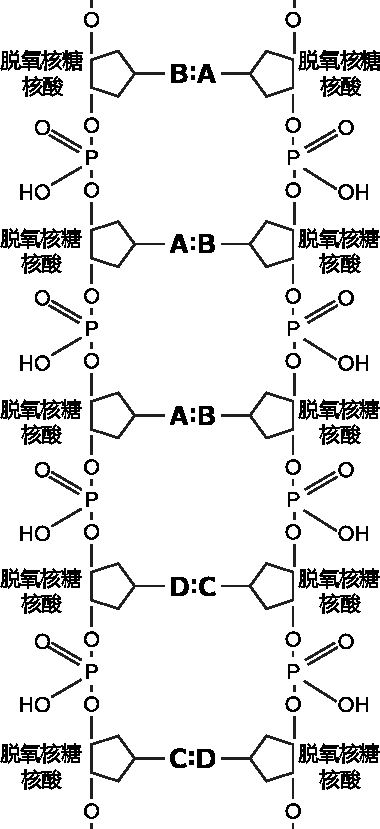
\includegraphics[width=0.48\textwidth]{部分DNA分子结构图}
\caption{部分DNA分子结构图}
\label{fig:部分DNA分子结构图}
\end{wrapfigure}

那么,复制又是怎么一回事呢?假设我们把这个整链一分为二,我们怎么能制造出另一个正好与它一样的链呢?如果在细胞的物质中有一种加工部门,产生了磷酸盐、糖以及没有联在一个链上的A、B、C、D单元,那么唯一能与我们那个分开的链相连的单元必须是正确的,是BAADC……的补体,即ABBCD……。于是,当细胞分裂时,链亦从中间裂开,一半最终与其中一个细胞在一起,而另一半则留在另一个细胞内;当它们分离后,每个半链都会形成一个新的补足的链。


接下来的一个问题是A、B、C、D单元的次序究竟怎样精确地决定蛋白质中氨基酸的排列?这是今天生物学中没有解决的一个中心问题。然而,初步的线索,或者说一点信息是:在细胞中存在一种叫做微粒体的小小粒子,现已知道它就是制造蛋白质的地方。但是微粒体并不在细胞核内,而DNA及它的指令却在细胞核内。看来是有某种原因的。然而,现在也知道从DNA分出的小分子,不像携带有全部信息的大DNA分子那样长,而像它的一个小部分。它叫RNA,但这无关紧要。RNA是一种DNA的拷贝——一个简短的拷贝。RNA不知怎么地携带了关于要制造那种蛋白质信息,跑到微粒体中,这一点我们已经知道了。当它到达那里后,在微粒体中就合成出蛋白质,这一点也已经知道了。不过,氨基酸是怎样进入蛋白质的,又是怎样根据RNA上的密码来排列,等等,这些细节则还不太清楚。我们不知道如何去解这种密码。比方说,假如我们知道了一排字母ABCCA,我们也无法告诉你要制造的是什么蛋白质。


今天,无疑没有一个学科或领域在这样多的前沿上比生物学取得更大的进展;如果我们要作出引导着人们在探索生命的努力中不断前进的最有成效的假说,这就是:\uwave{所有的物质都是由原子组成的},并且生命体所做的每一件事都可以从原子的摆动和晃动中来理解。


\section{天文学}
在我们对整个世界非常概括的描绘中,现在必须转到天文学上。天文学是一门比物理学古老的学科。事实上,正是天文学向物理学提出了解释星体运动的如此美妙而又简单的问题,对于这个问题的理解,就构成了物理学的\uwave{开端}。但是在所有的天文学发现中,最值得注意的是:\uwave{星体是用同地球上一样的原子组成的}\footnote{在这里我是讲得多么匆促啊!在这个简短的叙述中,每一句话包含了多么丰富的内容!“星体和地球部是用同样的原子组成的。”我通常挑选跟这一样的小题目来讲课。据诗人们说,科学使星星失去了美丽——它们只不过是由气体原子组成的球体。但事实上根本不是这么一回事。我同样会在荒凉的夜晚仰望星空,并且有所感受。但我是看得太少了还是太多了呢?无垠的天空丰富了我的想象,我那小小的眼睛扫遍这回转的天穹,就能注视这欢乐的天空,并且能够捕获一百万年前发出的里光。宇宙是一幅无边无际的图案——我也是其中的一部分——也许组成我的身体的材料正是从某个已被遗忘的星球上喷射出来的,就像那儿的一个星球正在不断爆发一样。假若我通过帕洛玛(Palomar)的巨大眼睛[指安装在美国威尔逊(Wilson)山帕洛玛天文台的200英寸光学望远镜——译者注。]来观察夜空,那么就会看到原来或许紧靠在一起的星群从某个共同的起点往四面八方奔驰而去。宇宙的模式,或者说它的含义,它的\uwave{成因}是什么?人们对这些问题有点了解是不会有损于宇宙的奥秘的。真理远比以往任何艺术家的想象更为奇妙!为什么现在的诗人不去歌颂它?如果朱庇特(木星)像一个人,诗人就会歌颂它,但是如果朱庇特是一个由甲烷和氨组成的旋转的巨大球体,诗人就很可能默不作声。}。那么这是怎么知道的呢?原子释放具有确定频率的光,这有点像乐器的音色是具有确定的音调或频率的声音。当我们听见几种不同的音调时,可以分别说出它们来,但是当我们用眼睛观察混合的颜色时,却无法说出它由哪几种颜色组成,因为眼睛的辨别能力在这一点上远远比不上耳朵。然而,利用分光镜我们\uwave{可以}分析光波的频率,这样就可以看见各个不同星体上的原子所发生的真正“音调”。事实上,有两种化学元素在地球上被发现之前就已经在星体上发现了。氦是在太阳上发现的,它的名称就是由此而来的;锝是在一种冷却的星体上发现的。这当然使我们在理解星体方面取得了一定的进展,因为它们也是用跟地球上同样的原子组成的。今天,我们已经知道了许多有关原子的知识,特别是它们在高温而密度不太大的条件下的行为,这样我们就能用统计力学的方法来分析星体物质的性能。即使我们无法在地球上复现有关的条件,但是应用基本的物理定律往往能精确地或十分接近地说出会发生什么事情。这就是物理学帮助了天文学。看来令人奇怪的是,我们对太阳内部物质的分布情况的了解远胜于对自己脚下的地球内部情况的了解。我们对星体\uwave{内部}发生的情况的了解要比在人们必须通过望远镜来观察小小的光点这种困难的情况下可能推测出更多一些,因为在大多数情况下,我们可以\uwave{计算}出星体里的原子应当做些什么。

给人印象最深的发现之一是使星球不断发出光和热的能量来源问题。有一个参与这项发现的人,在他认识到要使恒星发光,就必须在恒星上不断地进行核反应之后一天晚上和他的一位女朋友出去散步。当这个女朋友说:“看这些星星闪烁得多美啊!”他说:“是的,在此刻我是世界上唯一知道\uwave{为什么}它们会发光的人。”他的女朋友只不过对他笑笑。她并没有对于同当时唯一知道恒星发光原因的人一起散步产生什么深刻的印象。的确,孤单是可悲的,不过在这个世界上就是这个样子\footnote{呵呵,费曼先生。}。

正是氢原子核的“燃烧”给太阳提供了能量,这时氢也就转变成了氦。而且,最终从氢制造出各种化学元素的过程是在恒星的中心进行的。组成\uwave{我们}身体的各种元素在一个星体上一次“烹调”好后,就被抛出,存在于宇宙之中。我们是怎么知道的呢?因为这里有一条线索。\uwave{化学}反应永远改变不了不同的同位素的比例——多少\chemfig{C^{12}},多少\chemfig{C^{13}}等等,因为化学反应对二者而言都是大致相同的。这个比例纯粹是\uwave{核}反应的结果。看看,在熄灭的、冷却的余烬——比如我们自己就是这样的产物——里同位素的比例,就可以发现在构成我们身体的材料的形成时期\uwave{熔炉}象什么样子。这个熔炉很象恒星,所以很可能我们的元素是在恒星上“制造”出来,而在我们称为新星和超新星的爆炸中被喷吐出来的。正是因为天文学与物理学是这样密切相关,所以我们学下去时将要研究许多许多有关天文学的知识。



\section{地质学}
我们现存转到所谓的\uwave{地球科学}或\uwave{地质学}。首先是气象学和天气。当然气象学的\uwave{仪器}是物理仪器,就像前面所说的那样,实验物理学的发展使得提供这些仪器成为可能。然而,物理学家从来没有得出满意的气象学理论。“怎么!”你们会说:“这里除了空气以外什么东西都没有,而我们已经知道了空气的运动方程。”我们的确知道。“那么,如果我们知道了今天的空气状态,为什么就不能计算出明天的空气状态?”首先,我们并不\uwave{真正}知道今天的状态究竟是怎样的,因为空气到处旋转。结果它非常敏感,甚至不稳定。假如你们看到过水流平稳地流过水坝,然后当它下落时一下子变成大量的水珠和水滴的话,你就会懂得我所说的不稳定是什么意思了。你们知道水在流出溢水口之前的情况,它是十分平滑的;但是在它开始下落的一瞬间,水滴从哪里开始溅出?水滴将会有多大,并且在哪里的因素是什么?这些都无法知道,因为这里水是不稳定的。而对于空气来说,即使是平稳地运动着,但当它越过一座山时就变成了复杂的旋涡。在许多领域中都出现这种\uwave{湍流}现象,我们在今天还无法对之进行分析。现在,赶快离开天气问题,回到地质学上去吧!

对于地质学而言,它的基本问题是,究竟是什么使地球成为现在这个样子?最明显的过程就在你们眼前,这就是河流、风等等的侵蚀过程。要理解这些事是相当容易的,但是要知道,对于每一片侵蚀都有等量的另外一些东西出现。平均而言,今天的山脉并不比过去的低,因此必定有一种\uwave{造}山过程。假如你们学过地质学,你们就会知道,确实\uwave{存在}着造山过程以及火山作用,这些现象没有人懂得,但却占了地质学的一半内容。实际上,火山的本质并没有被人们所理解。造成地震的原因是什么最终也不了解。我们所知道的是,如果一个东西推动另外一些东西,那么就会突然断裂,并且产生滑动,这当然是对的。但是什么东西在推?为什么会这样?有一种理论认为,在地球内部存在着环流,它是由于内外温度上的差别而造成的,也就是它们在运动过程中轻微地推着地球的表层。这样假如有两股相对的环流在某个地方碰上的话,物质就会在这个区域里堆积起来而形成山脉,这些山脉处于非常不相宜的受到应力的状态,这样就会引起火山爆发,造成地震。

那么地球内部的情况是怎样的呢?关于地震波在地球里的传播速度以及地球的密度分布已经了解得很多。然而,关于物质处于我们预期在地球中心所应有的压强之下会有怎样的密度,物理学家没有能够提出一种有效的理论。换句话说,我们还不能很好地解决在这种情况下的物质的性质问题。我们在地球方面所做的事比在星体的物质条件下所做的事要差得多。这里所包含的数学到现在为止看来似乎过于复杂,但是也许不要很长时间就会有人认识到这是一个重要的问题,并且真正着手于解决这个问题。当然,另一方面,即使我们确实知道了密度,还是不能判断环流,也不能真正得知高压下的岩石的性质。我们无法说出岩石要多快才会“融化”;这必须通过实验来解决。


\section{心理学}
接下来,我们考虑\uwave{心理}科学。顺便提一下,心理分析并不是一门科学,它充其量不过是一个医学过程,也许更像巫术。\endnote{任何学科能够从数学上描述之后才能称之为真正意义上的科学,所以恕我直言,目前的中医西医都是医学,区别只有技术层面,但都算不上科学,他们对内部作用细节都没弄明白。}它有一个疾病起源的理论——据说有许多不同的“幽灵”等等。巫医有一个理论说像疟疾那样的疾病是由进入空气中的幽灵所引起的;但是医治疟疾的药方并不是将一条蛇在病人头上晃动,而是奎宁。所以,如果你的身体感到有什么不舒服,我倒劝你到巫医那儿去,因为他是对疾病知道得最多的那批人中的一个。然而,他的知识不是一种科学。心理分析没有用实验仔细地检验过,因此没有办法知道,在哪些情况下它是有效的,在哪些情况下则是无效的,等等。

心理学的其他一些分支,包括感觉的生理学——在眼睛里出现一些什么情况,在大脑中出现一些什么情况——可以说,是并不令人感到兴趣的。但是在它们的研究中取得了一些微小的然而是真正的进展。有一个最有趣的技术性问题可以归之为心理学,也可以不归之为心理学。即有关大脑——如果你愿意的话,或者说神经系统的中心问题是:当某种动物学到了某件事后,它就能做一些以前不会做的事,所以它的大脑细胞也一定会有变化——只要大脑细胞是由原子构成的。那么,\uwave{差别表现在哪里呢}?当一件事情被记在大脑里后,我们不知道在哪儿去找它,或者去找些什么东西。如果一件事情被学到了,它意味着什么,或者说神经系统有些什么变化,我们都不知道。这是一个很重要的问题,但根本没有解决。然而,假设存在着某种记忆的物质的话,那么大脑恰恰就是这么多的连线和神经的集合体,这种集合体大概是无法用简单的方式来分析的。这和计算机以及计算机单元很类似,它们也有大量的布线,有某种单元,大概就类似于神经元触点,或者说一根神经到另一根神经的联结点。思维和计算机之间的联系是一个非常有趣的课题,但我们在这里没有时间作进一步的讨论。当然,必须懂得这个课题在有关人们一般行为的真正复杂性上所告诉我们的东西是非常之少的。每个人之间存在着如此巨大的差别。为了要达到那种理解将需要很长的时间,我们必须把研究起点退到更后面的地方。假如我们总算能够解决\uwave{狗}是怎样活动的,我们就已经走得够远了。



\section{情况何以会如此 ?}
为了使物理学不仅在仪器的发明方面,而且在\uwave{理论}方面对其他科学也有所裨益,有关的科学就必须向物理学家提供用物理学家的语言描述的研究对象。人们或许会问:“青蛙为什么会跳跃?”物理学家对此就回答不出。如果人们告诉他青蛙是什么,这里有这么多的分子,那里有神经,等等,情况就不同了。假如人们或多或少地告诉我们地球或者星星是怎样的,那么我们就能够把它们想象出来。要使物理理论有点用处,我们就必须知道原子的位置。要理解化学,就应当确切知道存在着哪些原子,不然就无法分析。当然,这只是限制因素之一。

在物理学的姐妹科学中存在着另一\uwave{种}物理学中不存在的问题,因为没有更好的措词,我们可以称它为历史问题。情况何以会如此?假如我们懂得了生物学的一切,就会想要知道现在地球上的所有生物是怎样发展的。这就是生物学的一个重要部分——进化论。在地质学中,我们不仅要知道山脉正在怎样形成,而且要知道整个地球最初是怎样形成的,太阳系的起源,等等。当然,这就会使我们想要知道在宇宙的彼时有什么样的物质。恒星是怎样演化的?初始状态又是如何?这些都是天体的历史问题。今天我们已经弄清楚许多有关恒星的形成及有关组成我们身体的元素的形成的知识,甚至还知道一些有关宇宙起源的事。

目前在物理学中还没有这种历史问题要研究。我们不会问:“这里是物理学的定律,它们是怎样变化而来的?”我们此刻不去想象物理定律以某种方式随时间而变化,不认为它们在过去与现在是有差别的。当然,不能排除这种\uwave{可能},而且我们一旦发现果真如此时物理学的历史问题就将与宇宙发展的其余历史问题交织在一起,于是物理学家就要谈论天文学家、地质学家和生物学家同样的问题。

最后,在许多领域中普遍存在着一个物理问题,这是一个很古老的问题,但是还没有得到解决。这并不是寻找新的基本粒子的问题,而是好久之前——大约一百多年前就遗留下来的一件事情。在物理学上没有一个人能够真正令人满意地对它进行数学的分析,尽管它对于姐妹科学来说是一个重要问题。这就是\uwave{环流}或\uwave{湍流}的分析。如果我们注视着一个恒星的演化,就会发现这样的情形,我们可以推断出将要出现对流,但在这以后我们就再也无法推断会有什么事发生了。几百万年后这个星体会发生爆炸,但是我们想不出是什么道理。我们不能分析气候,也不知道地球内部的运动。这类问题的最简单的形式就是取一根很长的管子,使水高速通过。我们问:使一定量的水通过管子需要多大的压力?没有人能从基本原理和水的性质出发来分析它。如果水流得非常慢,或者用的是蜂蜜那样的粘性物质,那么我们可以分析得很不错。在你们的教科书上就有这方面的内容。我们真正不能处理的是实际的水流过管子的问题。这是一个我们有朝一日应当解决的中心问题,但是现在还没有解决。

有一位诗人曾经说过:“整个宇宙就存在于一杯葡萄酒中。”我们大概永远不可能知道他是在什么含义上这样说的,因为诗人的写作并不是为了被理解。但是真实的情况是,当我们十分接近地观察一杯葡萄酒时,我们可以见到整个宁宙。这里出现了一些物理学的现象:弯弯的液面,它的蒸发取决于天气和风;玻璃上的反射;而在我们的想象中又添加了原子。玻璃足地球上的岩石的净化产物,在它的成分中我们可以发现地球的年龄和星体演化的秘密。葡萄酒中所包含的种种化学制品的奇特排列是怎样的?它们是怎样产生的?这里有酵素、酶、基质以及它们的生成物。于是在葡萄酒中就发现了伟人的概括:整个生命就是发酵。任何研究葡萄酒的化学的人也必然会像巴斯德(L.Pasteur)所做过的那样发现许多疾病的原因。红葡萄酒是多么的鲜艳!让它深深地留在人们美好的记忆中去吧!如果我们微不足道的有限智力为了某种方便将这杯葡萄酒——这个宇宙——分为几个部分:物理学、生物学、地质学、天文学、心理学等等,那么要记住大自然是并不知道这一切的。所以让我们把所有这些仍旧归并在一起,并且不要忘记这杯酒最终是为了什么。让它最后再给我们一次快乐吧!喝掉它,然后把它完全忘掉!\footnote{此段甚美!}

\section{注释}
\showendnotes



\chapter{能量守恒}
\section{什么是能量}
讲完对事物的一般性描述后,从这一章起,我们开始比较详细地研究物理学中各个方面的问题。为了说明理论物理学中可能用到的概念和推理的类型,我们现在来考查能量守恒定律,它是物理学:最基本的定律之一。

有一个事实,如果你愿意的话,也可以说一条\uwave{定律},支配着至今我们所知道的一切自然现象。没有发现这条定律有什么例外——就我们所知,它是完全正确的。这条定律称为\uwave{能量守恒定律}。它指出,在自然界所经历的种种变化之中,有一个称之为能量的物理量是不变的。那是一个最抽象的概念,因为它是一种数学原理;说的是在某种情况发生时,有一个数量是不变的。它并不是一种对机制或者具体事物的描写,而只是一件奇怪的事实。起先我们可以计算某种数值,当我们看完了大自然耍弄的技巧表演后,再计算一次数值,其结果是相同的。(有点类似于在红方格中的象,移动了几步后——具体步骤并不清楚——它仍然在某个红方格里。我们这条定律就是这种类型的定律。)由于这是一种抽象的概念,我们将用一个比喻来说明它的含义。

设想有一个孩子,或许就叫他“淘气的丹尼斯(Dennis)”,他有一堆积木,这些积木是绝对不会损坏的,也不能分成更小的东西。每一块都和其余的相同。让我们假定他共有28块积木。每天早上他的母亲把他连同28块积木一起留在一个房间里。到了晚上,母亲出于好奇心很仔细地点了积木的数目,于是发现了一条关于现象的规律——无论丹尼斯怎样玩积木,积木数目仍旧是28块!这种情况继续了好几天。直到有一天她发现,积木只有27块了,但是稍许调查一下就发现在地毯下面还有一块——为了确信积木的总数没有改变,她必须到处留神。然而,某一天积木的数目看来有些变化,只有26块了!仔细的调查表明:窗户已经打开,再朝窗外一看,就发现了另外的两块积木。又有几天,经过仔细的清点表明总共有30块积木!这使她相当惊愕,以后才了解到布鲁斯(Bruce)这个孩子曾带着他的积木来玩过,并留了几块在丹尼斯的房间里。自从丹尼斯的母亲拿走了多余的积木,把窗关上,并且不再让布鲁斯进来以后,一切都很正常,直到有一次,她清点时发现只有25块积木。然而,在房间里有一个玩具箱,母亲走过去打开这个箱子,但是孩子大声叫喊道:“不,别打开我的箱子,”不让她打开玩具箱。这时母亲十分好奇,也比较机灵,她想出了一种办法,她知道—块积木重3英两,有一次当她看到积木有28块时曾经称过箱子的重量为16英两,这一次她想核对一下,就重新称一下箱子的重量,然后减去16英两,再除以3,于是就发现了以下的式子:
\begin{equation}
\label{Eq:I:4:1}
\text{(所见到的积木数)}
+
\frac{\text{(箱重)}-\text{$16$ 英两}}{\text{$3$ 英两}}=
\text{常数}.
\end{equation}
接着,又好像出现了某种新的偏差,但是仔细的研究又指出,浴缸里的脏水的高度发生了变化,孩子正在把积木扔到水里去,只是她看不见这些积木,因为水很混浊,不过在她的公式里再添上一项她就可以查明在水中有几块积木。由于水的高度原来是6英寸,每一块积木会使水升高\begin{LARGE}
$ \frac{1}{4} $
\end{LARGE}英寸,因而这个新的公式将是:
\begin{align}
\begin{pmatrix}
\text{见到的}\\
\text{积木数}
\end{pmatrix}&+
\frac{\text{(箱子重量)}-\text{$16$ 英两}}
{\text{$3$ 英两}}\notag\\
\label{Eq:I:4:2}
&+\frac{\text{(水的高度)}-\text{$6$ 英寸}}
{\text{$1/4$ 英寸}}=
\text{常数}.
\end{align}
在她这个复杂性逐渐增加的世界里,她发现了—系列的项来表示计算积木的方法,这些积木藏在不准她去看的那些地方。结果,她得出了\uwave{一个用于计算数量}的复杂公式,无论孩子怎样玩耍,这个量总是不变的。

这件事情和能量守恒有什么相似的地方呢?抽象地说,必须从这个图像中除去的最显著的一点就是,\uwave{根本没有积木}。在(\ref{Eq:I:4:1})及(\ref{Eq:I:4:2})中取走第一项,我们就会发现自己是在计算多少是有点抽象的东西。上述比较的相似之处在于以下几点。第一,当我们计算能量时,有时其中的一部分离开系统跑掉了,有时又有另一些能量进入这个系统。为了验证能量的守恒,必须注意我们没有把能量引入系统中或从系统中取走能量。第二,能量有许多\uwave{不同的形式},对每一种形式都有一个公式。这些不同形式的能量是:重力势能、动能、热能、弹性能、电能、化学能、辐射能、核能、质能。假如我们把表示这些能量的公式全都加在一起,那么,除非有能量逸出或有其他能量加入,否则其总和是不会改变的。

重要的是要认识到:在今天的物理学中,我们不知道能量究竟\uwave{是}什么。我们并不把能量想象成为以一定数量的滴状形式出现。它不是那样的。可是有一些公式可以用来计算某种数量,当我们把这些数量全部加在一起时,结果就是“28”——总是同一个数目。这是一个抽象的对象,它一点也没有告诉我们各个公式的机制或者\uwave{理由是}什么。


\section{重力势能}
只有当我们的公式包含了所有形式的能量时才能理解能量守恒。我想在这里讨论一下地球表面附近的重力势能的公式,并用一种与历史无关的方式来导出这个公式,这种推导方式只是为这堂课想出来的,也就是说一种推理思路,为的是要向你们说明一个值得注意的情况:从几个事实和严密的推理出发可以推断出很多有关大自然的知识。它也表明了理论物理学家投身于怎样的一类工作,我们这里的推理仿照了卡诺(Carnot)讨论蒸汽机效率时所使用的极其杰出的论证方式\footnote{事实上你们可能已经知道式(4.3),因此这一讨论的意义与其说是得出(4.3)式,不如说是表明能用推理论证的方法来得出这样的结果。}。

让我们考虑一种起重的机械,它有这样的特点:用降低一个重物的方法来提高另一个重物。此外还假设:在这种起重机械中\uwave{不可能有永恒的运动}。(事实上,根本不存在什么永恒运动,这正是能量守恒定律的一般表述。)在定义永恒运动时必须特别小心。首先,我们定义起重机械的永恒运动, 假如我们提起和放下一些重物并使机械回复到原来的状态后,发现最后的结果是\uwave{提升了一个重物},于是我们就有了永恒运动的机械,因为我们可以利用被提起的重物使另外的一些东西运转。这就是说,提起重物的机械\uwave{精确地}回到\uwave{原来的状态},而且是完全独立完成的——它没有从外界(就像布鲁斯的积木那样)取得能量来抬高这个重物。

图4-1所示是一台很简单的起重机械。这台机械举起三个单位的重物。我们把这三个单位的重物放在一个秤盘里,在另一个盘内则放置一个单位的重物。但是,为了使机械实际上能工作,我们必须在左边减去一点点重量。另一方面,我们可以通过降低三个单位的重物来升高一个单位的重物,只要我们在右边的盘子里提起一点点重量,当然,我们认识到,对于任何\uwave{实际}的起重机械来说,为了使它运行必须施加一点额外的作用。这一点我们暂时不去考虑。理想的机械并不需要额外的作用,然而它们事实上是不存在的。我们实际使用的机械在某种含义上可以说\uwave{几乎}是可逆的,即假如降低一个单位的重物能使这种机械提升三个单位的重物的话,那么降低三个单位的重物也能使这种机械把一个单位的重物提升到接近原来的高度。
\begin{fig}{简单的起重机械}
\label{fig:简单的起重机械}
\end{fig}
我们设想存在着两类机械:一类是\uwave{不}可逆的,它包括所有的真实的机械;另一类是可逆的。当然实际上它是不可能达到的,不管我们怎样仔细地去设计轴承、杠杆等等。但是,我们假设有这样的东西——一台可逆机;在它使一个单位(一磅或任何其他单位)重的物体降低一个单位距离的时候提起了三个单位的重物。把这台可逆机称为A机。假定它使三个单位的重物升高的距离是$ x $。此外,假设还有另一台机械——B机,它不一定是可逆机,并且也使一个单位的重物降低一个单位距离,不过使三个单位的重物升高的距离是$ y $。我们现在可以证明$ y $不会高于$ x $,这就是说,不可能建造这样一种机械,能把重物抬得比可逆机所提到的高度还要\uwave{高}。让我们来看看为什么是这样。假设$ y $大于$ x $。我们用B机使一个单位的重物降低一个单位距离,这使三个单位的重物升高距离y,然后,我们可以使这个重物从$ y $降到$ x $获得\uwave{自由的能量},再利用可逆机A反向运转,使三个单位的重物降低$ x $而使一个单位的重物升高一个单位距离。这样一个单位的重物回到了原来的高度,而使这两台机械又处于初始的备用状态!因此,假如$ y $高于$ x $,那么就会有永恒运动,但我们已经假设这是不可能的。于是利用这些假定,我们就能够推导出\uwave{$ y $不会比$ x $}高,因此在所有可能设计的机械中,可逆机是最好的。

我们还可以看出所有的可逆机提升的高度一定\uwave{完全相同}。假定B的确也是可逆的。当然,前面关于$ y $不会高于$ x $的论据现在同样成立,但是我们也可以把这两台机械的工作顺序倒过来,即反之论证$ x $不高于$ y $。这一点是很值得注意的,因为它使我们能够在\uwave{不考察内部机制}的情况下分析不同的机械对物体可以提升的高度。我们立刻知道,如果有一个人制作了一组极其精巧的杠杆,利用这组杠杆使一个单位的重物降低一个单位距离就可以把三个单位的重物提升到某一个高度,把这组杠杆和一个具有同样用途的简单的可逆的杠杆作比较就可以知道它不会比简单的可逆的杠杆提得更高,而是或许还会低一些。假如这个人的机械是可逆的,我们也能精确地知道它可以提得\uwave{多}高。概括地说就是:每一台可逆机械无论怎样运转,当它使一个单位的重物下降一个单位距离时,总是会使三个单位的重物提升同样的距离$ x $。很清楚,这是一条非常有用的普遍定律。接下来的问题自然是$ x $是多少?
\begin{fig}{一种可逆机}
\label{fig:一种可逆机}
\end{fig}
假如我们有一台可逆机,它能在3对1时提升距离$ x $。在图4-2中,我们在一个固定的多层架子上放置三个球。另外有一个球放在离地面一英尺的台上。这台机械可以使一个球降低1英尺来抬高三个球。现在,我们来这样安排:设容纳三个球的升降台有一层底板和两层架子,间隔正好是$ x $,其次,容纳球的多层架的间隔也是$ x $(图a)。首先我们使小球从多层架水平地滚到升降台上的架子中去(图b),我们假设这并不需要能量,因为高度并没有改变。于是开动可逆机进行工作:它使一个球降到底层,而使升降台升高距离$ x $(图c)。由于我们已经巧妙地安排了多层架,于是这些球又和架子相平。这样就把球卸到了多层架上(图 d)。卸了球以后,我们可以使机械回复到初始状态。现在在上面三层架子上有三个球,在底部有一个球,但是奇怪的是从某种观点上讲,我们根本没有使其中\uwave{两}个升高,因为,无论如何第二层和第三层架子像以前一样里面装着球。因此,最后的效果是使\uwave{一个}球升高了$ 3x$的距离。假如$  3x $超过1英尺,那么我们就可以把小球\uwave{放下来}使机械回到初始状态(图f),这样就能使这个装置再次运转。所以$ 3x $不可能超过1英尺,因为如果$ 3x $超过1英尺;我们就能创造出永恒运动。同样,使整台机械反向运行,我们可以证明,\uwave{1英尺不能超过$ 3x $},因为这是一台可逆机。所以\uwave{$ 3x $既不大于也不小于 1英尺},这样我们只是通过论证就发现了一条规律,$ x=\frac{1}{3} $英尺。显然,这条规律可以推广为:开动一台可逆机使1磅重物降下一定距离,那么这台机械可以使p磅重物提高那段距离的$ \frac{1}{p} $。另一种表示结果的说法是:3磅乘以所提高的距离(在我们的问题中是$ x $),等于1磅乘以所降低的距离(在这种情况下是1英尺)。如果我们先把所有的球的重量分别乘以它们现在所在的高度,然后使机械运转,再把所有的球的重量乘以它们所在的高度,得出的\uwave{前后结果不会有任何改变}。(我们必须把例子中只移动一个重物的情况推广到当我们降低一个重物就能提升几个不同的重物的情况——但这是不准的。)
\endnote{
整个过程就是假定球高度不变的平移过程是可逆的,然后左边一个球下降一定距离,那么将会引起右边的一个相同的球上升相同的距离,这个过程也是可逆。然后整个过程(左球下降,右球上升,左球填充下面的空位,上球滚到左边就绪等)是一个可逆的循环(类似卡诺循环)过程。前面我们证明了可逆过程是上升效率最高的过程,然后这里又证明了这个可逆过程上升的高度是和重量具有某种关系的。具体关系就是1磅下降3x那么3磅上升x,然后就有了下面引入的重力势能的基本定义。
}

我们把重量和高度的乘积之和称为\uwave{重力势能}——这是一个物体在空间上与地球之间的相互关系而具有的能量。那么,只要我们离地球不是太远(当位置很高时重力要减弱),重力势能的公式就是
\begin{equation}
\label{Eq:I:4:3}
\text{(一个物体的重力势能)}=
\text{(重量)}\times\text{(高度)}
\end{equation}
这是一条十分优美的推理思路。唯一的问题在于,或许这并不是实际的情形。(无论如何,大自然\uwave{毋须}按我们的推理行事。)例如,也许永恒运动事实上是可能的。某些假设可能是错误的,或者我们的推理或许有错误,所以验证总是必要的。事实上,实验证明它是正确的。

那种与别的物体的相对位置有关的能量的一般名称就称为\uwave{势能}。当然,在上面的特殊情况中,我们则称它为\uwave{重力势能}。如果我们克服电力做功,而不是克服重力做功,即用许多杠杆“提升”一些电荷使之离开其他的电荷,那么所包含的能量就称为电势能。一般的原则是能量的变化为有关的力乘以力所推过的距离,而且这是一般的能量变化:
\begin{equation}
\label{Eq:I:4:4}
\text{(能量的变化)}=
\text{(力)}\times\text{(力在作用下所通过的距离)}
\end{equation}
随着课程的进展我们还要讲到其余的种种势能。
\begin{fig}{斜面}
\label{fig:斜面}
\end{fig}

\begin{fig}{斯蒂维纽司的墓志铭}
\label{fig:斯蒂维纽司的墓志铭}
\end{fig}

在许多情况下能量守恒原理对于推断会发生什么事都是非常有用的。在高中你们已学过许多有关不同用途的滑轮和杠杆的定律,我们现在可以看到所有这些“定律”\uwave{都是一回事},并且不需要记住75条法则。一个简单的例子是如图4-3所示的一个光滑斜面,很巧,这是一个3--4--5的三角形。我们在斜面上用滑轮挂上一个1磅重的物体,而在滑轮的另一端悬挂一个重物$ W $。我们想知道为了平衡在斜面上的1磅重物,$ W $必须是多重?怎样来求出答案呢?假如我们说情况正好是平衡的话,那就是可逆的,因而可以使重物上下移动。所以,我们可以考虑下述情况。起初,如图(a)所示,1磅重物在斜面底部,而重物$ W $在斜面的顶端。当$ W $以一种可逆的方式滑下去后,1磅的物体就在斜面顶部,而$ W $经过的距离就是斜边的长度,如图(b)所示,即5英尺。我们使1磅重的重物只\uwave{提高}了3英尺而使W降低了\uwave{5英尺},所以,$ W=\frac{3}{5} $磅。注意,我们是从\uwave{能量守恒},而不是从力的分解来得出这个斯蒂维纽司(Stevinus)所发现的方法就铭刻在他的墓碑上。图4-4说明这个重物一定是$ \frac{3}{5} $磅,因为这个圆球链并没有转动,很明显链条的下端的部分是为自身所平衡的,所以一边三个重物的拉力必须与另一边五个重物的拉力平衡,即按边长的比例。从图中你们可以看到,W一定是$ \frac{3}{5} $磅。\endnote{就是直接数,假设斜面上五个球1磅,那么左边3个球一共$\frac{3}{5} $磅。}
\begin{fig}{螺旋起重器}
\label{fig:螺旋起重器}
\end{fig}
让我们现在用图4-5所示的螺旋起重器这个比较复杂的问题来说明能量守恒原理。螺旋的把柄长为20英寸,螺纹为每英寸10圈,我们想知道,为了举起一吨(2000磅)的重物,在把柄上要施加多大的力?假如我们要使一吨重物升高1英寸,就必须使把柄转10圈。把柄转一次时大约走过126英寸。所以它总共要走过1260英寸,如果我们利用各种滑轮之类的机械,就可以用加在柄的端点上的一个未知的小重物$ W $来举起1吨的重物,我们发现,$ W $大约是1.6磅。这就是能量守恒的一个结果。
\endnote{这里用到了能量的变化=力$ \times $力走过的距离的概念。}
\begin{fig}{一端支撑着的荷重杆}
\label{fig:一端支撑着的荷重杆}
\end{fig}
在图4-6中我们举一个稍为更复杂一点的例子。一根8英尺长的棒,一端被支撑着,在棒的中间有一个60磅的重物,离支点2英尺处有一个100磅的重物,假如不考虑棒的重量,为了保持它的平衡,我们要在棒的另一端加多大的力?假设在棒的那一端放上一个滑轮,并在滑轮上悬挂一个重物$ W $,为了使棒平衡,$ W $应当是多重?我们设想$ W $落下任意一段距离,为了简便起见,设它下降了4英寸,那么这两个重物要升高多少呢?棒的中心升高了2英寸,而离固定端2英寸处的那一点升高了1英寸,所以,各个重物与高度的乘积之和不变,这个原理告诉我们,$ W $乘以下降的4英寸,加上60磅乘以升高的2英寸,再加上100磅乘以升高的1英寸,其和必定是零。\endnote{这里是虚构的运动,所以可以假设移动很小一个角度,可以直接视作垂直向上运动。}
\begin{equation}
\label{Eq:I:4:5}
-4W+(2)(60)+(1)(100)=0,\qquad
W=\text{$55$ 磅}
\end{equation}
这就是说为了使棒平衡,必须加上一个55磅的重物。用这种方法,我们可以得出“平衡”定律——复杂的桥梁建筑的静力学,等等。这种处理问题的方法称为\uwave{虚功原理},因为为了进行这种论证,我们必须\uwave{设想}系统移动一下——即使它实际上没有移动,甚至不能移动。为了运用能量守恒的原理,我们用了很小的假想的运动。



\section{动能}
为了说明另一种形式的能量,我们来考虑一个单摆(图4-7)。
\begin{fig}{单摆}
\label{fig:单摆}
\end{fig}
假如我们把它拉向一边,再把它放开,它就会来回摆动。在这种运动中,每当从端点跑向中点时,它的高度降低了,这时势能跑到哪里去了呢?当摆降到底部时,势能就消失了,不过,它将再次爬上来。可见重力势能必定转变为另一种能量形式。很明显它是依靠了自己的\uwave{运动}才能重新爬上来。所以,当它到达底部时,重力势能就转变为某种其他形式的能量。

我们应当得出一个运动能量的公式。现在,回想一下关于可逆机的论证,很容易看出,在底部的运动必定具有一定量的能量,可使摆升高到一定高度,这个能量与摆上升的\uwave{机制}无关,或者说与上升的路径无关,所以与我们对孩子玩积木的情形所写出的公式一样,这里也有一个(两种能量间的)等价公式。我们有另一种表示能量的形式,要说明它是不难的。摆在底部的动能等于重量乘以它能升高的高度:\text{K.E.}= WH。现在需要的是一个利用某种与物体的运动有关的规则来说明摆动高度的公式。假如我们以一定的速度直接朝上抛出一个物体,它将到达一定的高度;我们暂时还不知道到底是多高,但是它依赖于速度——关于这个,有一个相应的公式。于是,为了找到物体以速度$ V $运动的动能的公式,我们必须计算它能到达的高度;再乘以物体的重量。我们立刻就会知道,可以把动能写成这种形式:
\begin{equation}
\label{Eq:I:4:6}
\text{K.E.}=WV^2/2g.
\end{equation}
当然,运动具有能量这个事实与物体处于重力场内这件事毫无关系。无论运动怎样产生,这都没有关系。这是一个适用于各种速度的一般公式。(\ref{Eq:I:4:3})及(\ref{Eq:I:4:6})两式都是近似的公式。(\ref{Eq:I:4:3})式在高度很大时是不正确的,因为这时,重力要减弱;而(\ref{Eq:I:4:6})在高速时要加以相对论性的校正。然而,当我们最后得到动能的精确公式时,能量守恒定律是正确的


\section{能量的其他形式}
我们可以继续以这种方法来说明能量还以其他的方式存在。首先考虑弹性能,假如我们拉伸弹簧,就必须作一些功,因为拉伸时,可以提起重物。所以弹簧在伸长的情况下具有做功的可能性。假如我们求出重量与高度的乘积之和,那将与总能量不符——我们必须加上另外的一些东西来说明弹簧处于拉紧状态这一事实。弹性能就是关于弹簧被伸长时这个事实的表述。它有多大呢?假如我们释放弹簧,那么弹簧经过平衡点时,弹性能就转变为动能,能量就在弹簧的伸长、压缩和动能之间来回变换。( 这里也有一些重力势能的增减,但是如果我们愿意的话,可以使实验“斜着”做)弹簧将一直来回振动,直到能量失掉为止……。啊哈!前面我们已经在整个过程中玩了一点小小的手法——如加上一些小重物使物体运动,或者说机械是可逆的,它们可以永远运动下去等。但是,我们可以看到这些东西最终都要停下来的。当弹簧不再上下振动时,能量到哪里去了呢?这就引进了另一种形式的能量:\uwave{热能}。

在弹簧或杠杆里有着由大量原子组成的晶体。假若极其仔细和精致地安排了机械的各个组成部分后,人们可以试着使事情作这样的调整:当某个东西在另一个东西上滚动时,根本没有一个原子会作任何跳动。但是我们必须非常小心。通常在机器运转时,由于材料本身的缺陷,会产生撞击和跳动,材料中的原子就开始无规则地摆动。于是那部分能量失踪了,但我们却发现机械运动减慢后,材料中的原子正以杂乱无章的方式摆动着,不错,这里仍然有动能,但是它与看得见的运动没有联系。多么奇怪!我们何以\uwave{知道}这里仍然有动能呢?我们发现,从温度计上可以看出,事实上弹簧或杠杆\uwave{变热}了,所以确实动能有了一定数量的增加。我们称这种形式的能量为\uwave{热能}。但是我们知道这实在并不是一种新的形式,它就是内部运动的动能。(我们在宏观范围内对物质所做的一切实验中都有一个困难,即不能真正演示出能量守恒,也不能实际制成可逆机,因为每当我们使大块材料运动时,原子不会绝对不受扰动,所以总有一定量的无规则运动进入原子系统,我们无法用眼睛看出这一点,但是可以用温度计或其他方式测量出来。)

还有许多其他形式的能量,当然,眼下不可能对它们叙述得更详细些。这里有电能,它与电荷的吸引和排斥有关。存在着一种辐射能,即光能,我们知道它是电能的一种,因为光可以表示为电磁场的振动;还有化学能——在化学反应中释放的能,它是原子彼此间相互吸引的能量。弹性能也是如此,所以实际上,弹性能在一定程度上就像化学能。我们目前对化学能的理解是化学能可分为两部分:首先是原子内电子的动能,所以化学能的一部分是动能,其余一部分是电子和质子的相互作用所产生的电能。接下去我们来考虑核能,它涉及原子核内的粒子的排列。我们有核能的公式,但是没有掌握基本的定律。我们知道它不是电能,不是重力能,也不纯粹是化学能,但是不知道它究竟是什么。看来这是另外的一种能量形式;最后,存在着一个与相对论有关的对动能定律的修正(或者你喜欢用的随便哪一种说法),也就是说动能与另一种称为\uwave{质能}的东西结合在一起。一个物体由于它的纯粹的\uwave{存在}就有能量产生。假如有一个静止的电子和一个静止的正电子起先稳定地搁置着而不发生任何作用——既不去考虑引力效应,也不去考虑其他,然后当它们碰在一起时就会湮没,并释放出一定量的辐射能,它是可以计算的。为此我们需要知道的只是物体的质量,而与究竟是什么物体无关。两个粒子消失后,就产生了一定的能量。爱因斯坦首先找到了计算公式,即$ E=mc^2 $。

从我们的讨论中可以很明显地看到,在进行分析时,能量守恒定律是极其有用的。我们已经在几个例子中表明了这一点,在那些例子中并没有知道所有的公式。假如我们有了各种能量的公式,那么毋须深入细节就能分析出有多少过程应当会发生。所以守恒定律是非常有趣的。由此很自然会产生一个问题,在物理学中还有哪些其他守恒定律?有另外两条守恒定律是与能量守恒定律类似的,一条称为线动量守恒,另一条称为角动量守恒,关于这方面我们在以后会知道得更多。归根到底,我们并没有深刻地理解守恒定律。我们不理解能量守恒,并不认为能量是一定数量的滴状物。你们也许听说过光子是以一个个的滴状形式出现的,一个光子的能量是普朗克常数乘以频率。这是正确的。但由于光的频率可以是任意的,所以没有哪条定律断言能量必须是某种确定的数值。与丹尼斯的积木不同,能量的数值可以是任意的,至少今天的理解是如此。所以在目前我们并不把能量理解为对某种东西的计数,而只是看作一种数学的量。这是一种抽象而又十分奇怪的情况。在量子力学中,我们知道能量守恒与世界的一个重要性质——事物不依赖于绝对时间——有十分密切的关系。我们可以在一个给定的时刻安排一个实验,并且完成它,然后在晚一些的时候再做同样的实验,那么实验的情形将完全是相同的。但这是否严格正确,我们并不知道。如果我们假设它\uwave{是}正确的,再加上量子力学的原理,我们就可以推导出能量守恒定律,这是一件相当微妙和有趣的事,不容易加以解释。其他的守恒定律也有联带的关系。动量守恒定律在量子力学中与一个命题有关,即无论你在\uwave{哪里}做实验都不会造成什么差别,结果总是同样的。最后,像空间上的无关性与动量守恒相联系、时间上的无关性与能量守恒相联系一样,假如我们\uwave{转动}仪器的话,这也不会造成任何差别,所以世界在角度取向上的不变性与\uwave{角动量守恒}相关。此外,还有三条其他的守恒定律。迄今为止我们可以说,这些定律是精确的。它们要容易理解得多,因为在本质上它们是属于清点积木一类的事。

这三条守恒定律中的第一条是电荷守恒定律这只是意味着,数一下你有多少正电荷,多少负电荷,将正电荷的数量减去负电荷的数量,那么这个结果将永远不会改变。你们可以用一个负电荷抵消一个正电荷,但是你们不可能创造任何正电荷对负电荷的净余额。另外两条守恒定律与这一条相类似。一条称为\uwave{重子的守恒}。存在着一些奇异粒子,例如中子和质子,它们称为重子。在任何自然界的反应中,假如我们数一下有多少重子进入一个反应,那么在反应结束时出去的重子\footnote{反重子的重子数记为(-1)}的数量将完全相同。还有一条是轻子守恒定律。我们可以举出称为轻子的一群粒子:电子,μ介子和中微子,还有一个电子的反粒子,即正电子(轻子数为-1)。在一个反应中对轻子的总数进行计数将揭示出这个事实:进入的数量与出去的数量决不会改变,至少就今天所知就是如此。

这就是六条守恒定律,其中三条是微妙的,与空间和时间有关,另外三条从对某种东西进行计数的意义上说是简单的。

关于能量守恒,我们应当指出,可资利用的能量是另一回事——在海水中的原子进行着大量的晃动,因为海水具有一定的温度,但是如果不从别处取得能量,就不可能使原子都按一个确定的方向运动。这就是说:虽然我们知道能量确实守恒,但是可供人类利用的能量并不那么易于保存。确定究竟有多少能量可供利用的那些定律称为\uwave{热力学定律},它们包括着一个称为熵的有关不可逆热力学过程的概念。

最后,我们提一下这个问题:今天我们可以从哪里获得能量的供应?我们的能量来源是太阳、雨水、煤、铀以及氢。大阳形成了降雨,也造成了煤矿,所以所有这些都起源于太阳。虽然能量是守恒的,但看来大自然对此并无兴趣,她使太阳释放了大量的能量,但其中只有二十亿分之一到达地球。大自然保存着能量,不过实际上并不关心这一点;她让巨大数量的能量向四面八方散布开去。我们已经从铀中得到能量,从氢中也能得到能量,但是,现在只是在爆炸的危险的条件下才得到这些能量。假如可以在热核反应中控制它,那么结果每秒钟从10夸脱水中得到的能量就等于整个美国每秒钟所发的电量,每分钟用150加仑的水,就会使你们有足够的燃料来供应今天在整个美国所需要使用的能量!所以,怎样想出一些办法使我们从对能量的需要中解放出来就成为物理学家的责任。无疑,这是可以达到的目标。

\section{注释}
\showendnotes



\chapter{时间与距离}
\section{运动}
在这一章里我们将研究\uwave{时间}和\uwave{距离}这两个概念的某些方面。上面我们曾经强调过,物理学像所有其他科学一样是依赖于观察的,人们或许还可以说,物理科学发展到它今天这种形式在很大程度上是由于强调了要进行\uwave{定量的观察}。唯有通过定量的观察,人们才能得到定量的关系,这些关系是物理学的核心。

很多人都喜欢把伽利略在350年前所做的工作看作是物理学的开端,并且称他为第一个物理学家。在此之前,对运动的研究是一种哲学上的事情,它所根据的是人头脑中所能想象出来的一些论据。大部分的论据是由亚里士多德和其他希腊哲学家提出的,并且被认为是“已经证明”了的。伽利略采取一种怀疑的态度,关于运动他做了一个实验,这个实验主要是这样的:他让一个球沿一斜面滚下,并且观察它的运动。然而他并不只是观察而已,而且还测量了在\uwave{多长一段时间}内小球跑了\uwave{多远一段距离}。

在伽利略之前很久,人们已经很好地掌握了测量距离的方法,但是,对于时间的测量,特别是短时间的测量,还没有精确的方法。虽然伽利略后来设计了比较准确的钟(不过不像我们今天所见到的那样),但他在第一次做运动实验时是用他的脉搏来数出等间隔的时间。让我们也来做一下这个实验。
\begin{fig}{一个小球沿着斜面滚下}
\label{fig:一个小球沿着斜面滚下}
\end{fig}
当小球沿着轨道滚下时(图5-1),我们可以数自己的脉搏:\\“一…二…三…四…五…六…七…八…。”我们请一个朋友于每数一次就在小球所到达的位置上做一个小记号;然后就可以测量小球从被释放的位置开始在1个、2个或3个等等相等时间间隔内所经过的\uwave{距离}。伽利略用下面这种方法来表述\uwave{他的}观察结果:如果从小球释放的时刻算起,它的位置是在1,2,3,4,……单位时间记下的,那么这些记号离开起点的距离就正比于数1,4,9,16,……。今天我们就会这样说:距离与时间的平方成正比:
\begin{equation*}
D\propto t^2.
\end{equation*}

\uwave{运动}的研究对所有物理部门是一件基本的事,它所讨论的问题是何处与何时?



\section{时间}
让我们先来考察一下何谓\uwave{时间}。时间究竟是什么?假如我们能够找到时间的一个确切的定义那该是多好。在韦伯斯特辞典里把“一段时间(a time)”定义为“一个时期(a period)”,又把后者定义为“一段时间”。这种定义看来并不十分有用。或许我们应该说:“时间就是不发生其他事情时所发生的事。”然而这也未必使我们的理解深入。事实上(就字典的含义来说) 时间很可能是我们不能定义的事物之一。面对这个事实也许并没有什么不好。我们干脆说时间就是我们所知道的那回事:它就是我们等了多久!

不管怎样,重要的不在于我们是如何来\uwave{定义}时间,而在于我们如何来测量它 测量时间的一种方法是利用某种能以有规则的方式一再发生的事情,即某种能\uwave{周期性}发生的事情。例如,一个昼夜。昼夜似乎是一再重复出现的。然而你思索一下,也许就会问:“昼夜是否系真正周期性重复的?它们是否有规则地变化着?每一天是否都同样长?”人们肯定会有这种印象,夏天的日子比冬天的日子长。当然,在人们感到非常无聊的时候,总觉得冬天的有些日子长得可怕。你们一定会听到过有人这么说:“哎呀,这是多么长的一天!”

但是\uwave{就平均而言},日子确实大致一样长。我们有没有什么方法来检验日子——不论从一天到下一天,或者至少就其平均而论——长短相同与否?一个办法是把它同某种别的周期性现象作比较,我们来看怎样能用一个沙漏来做这种比较。如果我们让某个人昼夜站在它的旁边,每当最后一粒沙掉下之后,他就把沙漏倒转来,这样,我们用沙漏就能“创造”一个周期性的事件。

于是,我们就能计算从每天早上到下一天早上倒转沙漏的次数,这一次我们大概会发现每一“天”的“小时”数(即倒转沙漏的次数)并不相同。这样,我们就会猜疑太阳或者沙漏,或者怀疑这二者。在加以思索之后,我们或许会想到要计算从这个中午到下一个中午的“小时”数。(在这里中午的定义并不是12:00,而是指太阳在其最高点的时刻。)这一次我们将会发现,每一天的小时数都是相同的。

现在我们比较有把握认为“小时”和“昼夜”具有一种有规则的周期性,也就是说它们划分出相继的等时间间隔,虽然我们没有\uwave{证明}它们中不论那一个“确实”是周期性的。或许有人会问:是否会有某个万能者在夜间使沙漏中的流动变慢,而在白天又把它加快?我们的实验当然无法对这类问题做出回答,我们所能说的,只是发现一种事物的规则性与另一种事物的规则性相吻合而已。我们只能说把时间的\uwave{定义}建立在某种明显是周期性的事件的重复性上。


\section{短的时间}
现在我们要指出,在检验昼夜的重复性这个过程中我们获得了一个重要的副产品。这就是找到了一种比较精确地测量一天的\uwave{几分之一}的方法。亦即我们找到了一种用较小的间隔来计点时间的方法。能不能把这种过程再往前发展,从而学会测量甚至更小的时间间隔呢7  。

伽利略断定,只要一个摆的摆幅始终很小,那么它将总以相等的时间间隔来回摆动。如果做这样一个实验,对摆在一“小时”内的摆动次数进行比较,那么这个实验就会表明,情况确实如此。我们用这个方法可划分出一个小时的\uwave{几分之一}。假如我们利用一个机械装置计点摆动次数,并且保持摆动进行下去,那么就得到了我们祖父一代所用的那种摆钟。

让我们约定,如果我们的摆一小时内振动3600次(并且如果一天有24个这样的小时),那么我们就称每一摆动的时间为1“秒”。这样,就把原来的时间单位分成大约$ 10^5 $个部分。我们可以应用同样的原理把秒分成更加小的间隔。你们可以理解,制造一个能够走得任意快的机械摆是不现实的,但是我们现在能够制造一种称为振荡器的\uwave{电学摆}。这种电学摆能提供周期很短的摆动。在这种电子振荡器中,是电在来回振动,其方式与摆锤的摆动方式相类似。

我们可以制造一系列这种电子振荡器,每一个的周期要比前一个减小10倍。每一个振荡器可用前一个较慢的振荡器这样来“定标”,即数出较慢的振荡器振动一次时它所振动的次数。当我们的钟的振动周期小于一秒的几分之一时,如果没有某种辅助装置以扩展我们的观察能力,那就无从计点振动的次数。这种装置之一是电子示波器,它的作用就像一种供短的时间用的“显微镜”。这个装置在荧光屏上画出一幅电流(或电压)对时间的图像。将示波器依次与我们的系列中相继的两个振荡器相连,它就先显示出一个振荡器中的电流图像,然后显示出另一个振荡器中的电流图像,从而得到如图5-2所示的两幅图像。这样,我们就很容易测出较快的振荡器在较慢的振荡器的一个周期中振动的次数。
\begin{figure}[H]
\centering
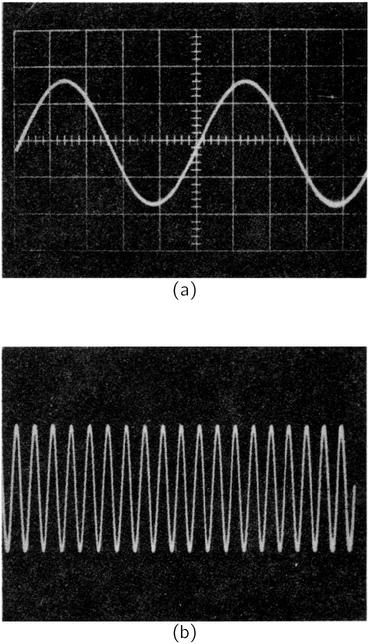
\includegraphics[scale=3 , keepaspectratio]{示波器屏上的两个图象}
\caption{\footnotesize 示波器屏上的两个图象。在(a)中,示波器与一个振荡器相连接;在(b)中,它与另一个其周期只有前者十分之一的振荡器相连接。}
\end{figure}


利用现代电子技术,已经制造出周期短到大约$ 10^{-12} $秒的振荡器,并且可以按照前面描述的那种比较方法用我们的标准时间单位——秒来予以定标。近年来,随着“激光器”或光放大器的发明和完善,已能制造周期甚至比$ 10^{-12} $秒更短的振荡器了,但是还不能用上述那些方法来予以定标,虽然毫无疑问,这在不久期间一定能够做到。

比$ 10^{-12} $秒还短的时间已经测量出来,但用的是另一种测量技术。事实上,这里所用的是“时间”的另一种\uwave{定义}。一个方法是观察发生在运动物体上的两个事件之间的\uwave{距离}。例如,假定有一辆行驶的汽车把它的车灯先开亮,然后再关掉。如果我们知道车灯开、关的\uwave{地点},以及车速,那么我们就能求出灯开的时间有多长。这段时间就是灯开时所通过的距离除以汽车的车速。

近几年来,正是这种技术被用来测量$\pi^0$介子的寿命。$\pi^0$介子在感光乳剂中产生并在其中留下微细的踪迹,用显微镜观察这些踪迹时,人们就可看到,平均而言一个$\pi^0$介子(认为它以近于光速的某个速度运动)在蜕变之前大约走过了$ 10^{-7} $米的距离,所以它的寿命总共只有大约$ 10^{-16} $秒。但是必须着重指出,这里我们用了一个与前稍有不同的“时间”的定义。然而,只要在我们的理解方面不出现任何不协调的地方,那么我们就觉得有充分的信心认为这些定义是足够等效的。

在把我们的技术——而且如有必要也把我们的定义——进一步加以扩展之后,就能推断更快物理事件的持续时间,我们可以谈论原子核振动的周期,以及第二章中提到过的那种新发现的奇异共振态(粒子)的寿命。它们的全部寿命只不过占$ 10^{-24} $秒的时间,大致相当于光(它以我们已知的最快速度运动)通过氢原子核(这个已知的最小物体)所花的时间。

那么,再短的时间呢?是不是还存在尺度更小的“时间”?如果我们不能够测量——或者甚至合理地去设想——某些发生在更短时间内的事情,那么要谈论更短的时间是否还有任何意义?可能没有意义。这是一些尚未解决的、但你们会提出的、而且也许在今后二十或三十年内才能回答的问题。


\section{长的时间}
我们现在来考虑比一昼夜还长的时间。要测量较长的时间很容易,我们只要数一数有几天就是——只要旁边有人在做这种计数的工作。首先我们发现,自然界里存在着另一个周期性,即年,一年大约等于365天。我们还发现,自然界有时也为我们提供了计算年的一些东西,例如树木的年轮或河流底部的沉积物。在某些情况下,我们就能利用这些自然界的时间标记来确定从发生某种事件以来所经历的时间。

当我们不能用计算年的方法来测量更长的时间时,那就必须寻找其他的测量方法。最成功的方法之一是把放射性材料作为一只“钟”来使用。在这种情况下,并不出现像昼夜或摆那样周期性的事件,但是有一种新的“规则性”。我们发现,某种材料的样品,当它的年龄每增加一相同的数值时,它的放射性就减少一相同的\uwave{分数}。假如我们画一张图来表示所观察到的放射性作为时间(比方以天来计算)的函数,那么我们就得到如图5-3所示的一条曲线。
\begin{figure}[H]
\centering
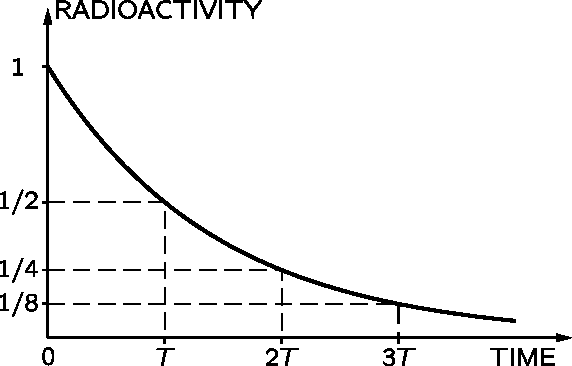
\includegraphics[scale=1 , keepaspectratio]{放射性随时间而减少}
\caption{\footnotesize 放射性随时间而减少。在每一个“半衰期”$ T $中,放射性都减少一半}
\end{figure}
我们看到,如果放射性在$ T $天内减少到一半(称为“半衰期”),那么它在另一个$ T $天内就减少到四分之一等等。在任一时间间隔$ t $内共包含了$ t/T $个半衰期,而在这段时间$ t $后尚剩下的部分则是$ (\tfrac{1}{2})^{t/T} $。

如果我们知道一块材料比如说一块木料,在它形成时其中含有数量为$ A $的放射性物质,而用直接测量我们发现它此刻的量为$ B $,那么只要解方程
\begin{equation*}
(\tfrac{1}{2})^{t/T}=B/A.
\end{equation*}
就能计算这一物体的年龄$ t $。

幸运的是,在某些情况中,我们可以知道物体在形成时它所包含的放射性总量。比如说我们知道空气中的二氧化碳含有某一确定小量的放射性碳同位素C$ ^{14} $(它由于宇宙线作用而连续不断地得到补充),如果我们测量一个物体的碳的总含量,并且知道这个总含量的某一分数原来是放射性的C$ ^{14} $,那么,我们就知道上述公式中所要用到的那个开始时的总含量$ A $ 。碳14的半衰期是5000年,通过仔细的测量我们测出经20个左右的半衰期后所余留下来的数量。因此,我们就能够确定生长于100,000年以前那样古老的有机体的年代。

我们很想知道,并且认为也能知道比之更老的那些事物的寿命。许多有关这方面的知识,我们是通过测量具有不同半衰期的其他放射性同位素而得到的。如果我们用一种半衰期更长的同位素来进行测量,那么就能测得更长的时间。例如,铀有一种同位索,它的半衰期大约为$ 10^9 $年,所以如果有一种物质在它$ 10^9 $年前形成时就含有这种铀,那么今天这种铀就只剩下一半。当铀蜕变时,它变成了铅。设想有一块岩石,它是在很久以前通过某种化学过程形成的。铅由于具有与铀不同的化学性质,它将出现在岩石的一个部分中,而铀则出现在岩石的另一部分中。铀和铅将互相分开。如果我们今天来考察那块岩石将发现在那种应该只有铀存在的地方,现在有某一分数的铀和某一分数的铅,通过对这两个分数的比较;我们就能说出百分之几的铀已消失并且变成了铅。利用这个方法,有些岩石的年龄被测定为几十亿年。这个方法的一个推广便是不用特定的岩石,而是着眼于海洋中的铀和铅,并且对整个地球取其平均值。用这个推广了的方法(在过去几年中)曾测得地球本身的年龄为大约55亿年。

人们发现,地球的年龄与掉到地球上的陨石(也是用铀方法测定的)的年龄是相同的,这是一件令人鼓舞的事情。看来,地球是由漂游在太空中的岩石形成的,而陨石很可能就是遗留下来的那些物质的残片。在50亿年前的某个时候,宇宙开始形成。现在人们认为,至少我们这部分宇宙起源于大约100或120亿年之前。我们不知道在此之前发生过什么事情。事实上我们又可以提出来问:这个问题是否有任何意义?更早的时间是否有任何意义?


\section{时间的单位和标准}
我们在前面实际上已表明了,如果从时间的某个标准单位,比如一天或一秒出发,并把所有其他的时间表示为这个单位的倍数或分数,那么将十分方便。然而,我们将用那个单位作为我们的时间基本标准呢?是否用人的脉搏跳动?如果我们比较各人的脉搏,那就会发现它们之间似乎差别很大。如果比较两只钟,则发现它们的变化不那么大。于是你们会说:好,就让我们采用钟吧!但是用谁的钟呢?有个故事讲到一个瑞士男孩,他想使他所在的镇上所有的钟在正午时刻都同时敲响,所以他就跑来跑去,穿家过院,想使人人相信这样做的好处。每个人都想,如果他的钟在正午敲响时,其他钟也全都敲响的话,这该是一个多好的主意呀!然而要决定谁的钟应该取作标准,这倒是一件难事。幸运的是,我们大家都同意用一只钟,即地球。在很长一段时间里,人们把地球的自转周期当作时间的基本标准。但是当测量越来越变得精确的时候,人们发现,用最好的钟来进行测量,地球的转动也不是严格周期性的。我们有理由相信,这些“最好”的钟是精确的,因为它们彼此之间是相符的。由于种种理由,我们现在认为,有些天要比另一些天长,有些天要比另一些天短,平均而论,地球的自转周期是随着一个世纪一个世纪的过去而变长了一点的。

直到晚近以前,我们还没有找到任何一个比地球的周期好得多的标准,所以把所有的钟同一天的长度联系了起来,而把一秒规定为一个平均日的$  1/86400$。最近我们对自然界中某些振荡器获得了一些经验。我们现在相信,这些振荡器可以当作比地球更稳定的时间参考物。而且,它们也是基于一个大家都能采用的自然现象。这就是所谓的“原子钟”。它的基本的内在周期,就是原子振动的周期,这种振动对于温度或任何其他外界影响都不十分敏感。原子钟能使时间的精确度达到$ 10^9 $分之一,或者比之更高。在过去二年中,哈佛大学的拉姆齐(N.Ramsay)教授研制了一种改进的原子钟,它是依靠氢原子的振动而工作的。拉姆齐认为,这种钟比其他原子钟精确100倍。现在他正在对之作测量,这些测量将表明他的说法是否正确。

既然现在有可能制作远比天文时间精确的钟,那么我们可以预期,科学家们不久就会一致同意采用许多原子标准钟中的一种来定义时间单位\footnote{1967年的第十三届国际计量大会已通过决议将时间单位“秒”的定义改为:“一秒等于铯133原子基态的两个超精细能级之间跃迁的辐射周期的9,192,631,770倍。”——译者注。}



\section{长的距离}
现在我们转到\uwave{距离}的问题上来。事物有多远,或者有多大?人们都知道测量距离的方法是选用一种长度单位再加上计数,例如可以用尺或拇指边量边数。那么怎样来量比较小的东西呢?怎样把距离分小呢?这与我们将时间分小一样,我们同样取一个较小的单位,然后数出这个单位组合成一个较长单位时所需的数目。这样我们就能测量越来越小的长度。

但是我们并不总是把距离理解为用米尺量。得的结果。仅仅用一根米尺是难以测量两个山顶之间的水平距离的。我们曾经凭经验发现可以用另一种方式来测量距离:即用三角法。
\begin{fig}{用三角法测定人造卫星的高度}
\label{fig:用三角法测定人造卫星的高度}
\end{fig}
虽然这意味着我们实际上对距离用了一个不同的定义,但当它们可以一起应用时,就应是彼此相一致。空间或多或少有点像欧几里得所设想的那个样子,所以距离的这两种定义是一致的。既然它们在地球上相一致,那就使我们充满信心可用三角法来测量更大的距离。例如,我们当时曾用三角法测定了第一颗人造卫星的高度(图5-4)。我们测得的高度约有$ 5\times 10^5$米。如果测量得更仔细一点,则用同样的方法可以测出地球到月球的距离;安放在地球上两个不同地点的两个望远镜,将会告诉我们所需要的两个角度。用这种方法我们求得月球离我们有$ 4 \times 10^8 $米远。

对于太阳,我们不能这样做,或者至少到现在没有人能够这样做。由于我们不能相当精确地对准太阳上一个特定的点,从而不能精确地测出两个角度,所以无法测出到太阳的距离。然而如何来测量这个距离呢?我们必须将三角法这个观念加以引伸。我们可以通过天文观察方法来测量所有行星出现的位置之间的相对距离,从而得到一幅有关太阳系的图像,能显示每个行星间的相对距离,但都不是绝对距离。因此需要测出一个\uwave{绝对}距离,而这种绝对测量已用几种方法得到,其中直到最近以前还认为最精确的一个是测出地球到爱神星的距离。爱神星是一个时常靠近地球的小行星。如果对这个小天体应用三角法,就能得到一个所需要的比例尺度。由于知道了其他天体的相对距离,我们就能说出它们之间的绝对距离,例如地球到太阳,或地球到冥王星的绝对距离。

去年,我们在有关太阳系的比例尺度的了解上获得了巨大的进展。喷气推进实验室用直接的雷达观察非常精确地测定了地球到金星的距离。当然,这只是另外一种由推测而得到的距离。我们说,我们知道光传播的速度(因而这也是雷达波传播的速度),并且假定,在地球与金星之间无论何处这个速度都相同。那么,在发射无线电波并测得电波返回的时间,我们就能从\uwave{时间}来推测\uwave{距离}。这确实是距离测量的另一种定义。

可是我们如何来测量一个更遥远的恒星的距离呢?幸运的是,我们可以回到三角法上来,因为地球绕太阳公转,而这种转动就为测量太阳系外的恒星距离提供了一条基线。假如我们在夏天和冬天用望远镜对准一颗恒星,那么我们可以期望能足够精确地测出这两个角度,从而能测出地球到恒星的距离。
\begin{figure}[H]
\centering
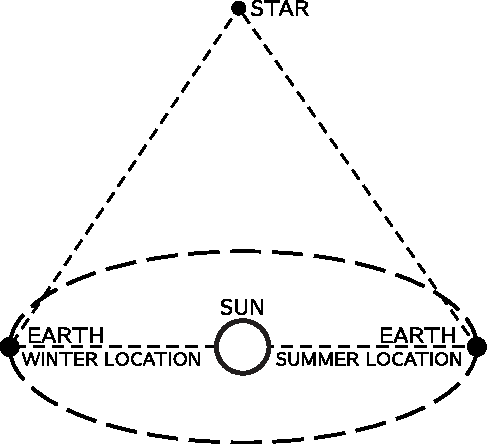
\includegraphics[scale=1 , keepaspectratio]{三角法测量恒星距离}
\caption{\footnotesize 利用地球轨道的直径作为基线,可以用三角法测量靠近地球的恒星的距离}
\end{figure}

如果恒星离得太远而不能应用三角法时又怎么办?天文学家总是在发明测量距离的新方法。例如,他们发现,从恒星的颜色可以估计它的大小和亮度。他们测定了许多靠近地球的恒星——这些恒星的距离已用三角法测得——的颜色和内在亮度,并且发现在恒星颜色和内在亮度(在大多数情况中)之间存在着一个平滑的关系,如图5-5所示。如果现在测出了一个遥远恒星的颜色,那就可以用颜色—亮度关系来确定这个星体的内在亮度,在测量了我们地球上看来这颗恒星有多亮(或许应该说有多\uwave{暗})之后,我们就可以计算它有多远(对于一个给定的内在亮度,其表观亮度是随距离的平方而减小的)。对称为球状星团的一群恒星作测量后,所得的结果很好地证实了这种星际距离测量方法的正确性。图5-6是这样一群恒星的一张照片。只要看一下照片,人们就会相信这些恒星都聚集在一起。用颜色—亮度关系这个测量距离的方法得到了同样的结果,
\begin{figure}[H]
\centering
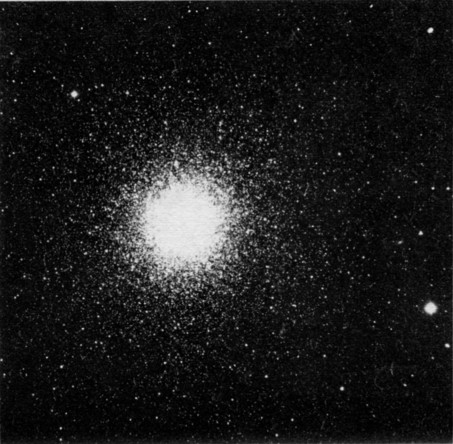
\includegraphics[scale=2.5 , keepaspectratio]{靠近我们银河系中心的一个星团}
\caption{\footnotesize 靠近我们银河系中心的一个星团,其中各恒星与地球的距离为30,000光年,或约$ 3\times 10^{20} $米}
\end{figure}

对许多球状星团进行研究之后使我们得到另一些重要信息。人们发现,在天空的某一部分有许多这样的星团高度集中在一起,而且其中大部分离地球的距离大致相同。把这个信息和其他证据结合起来,就能断定,星团的这个集中处就是我们所在银河系的中心。于是我们就知道到银河系中心的距离——大约为$ 10^{20} $米。

知道了我们自己所在银河系的大小,我们就有了一把测量更大距离——也就是到其他银河系的距离——的钥匙。图5-7是一副形状与我们的银河系颇为相同的一个银河系的照片。
\begin{figure}[H]
\centering
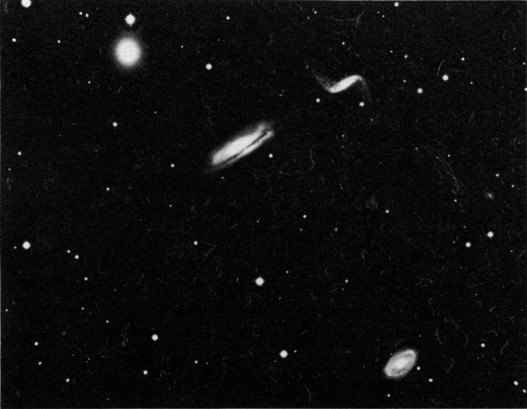
\includegraphics[scale=2.5 , keepaspectratio]{和我们银河系一样的一个螺旋银河系}
\caption{\footnotesize 和我们银河系一样的一个螺旋银河系,假定它的直径与我们银河系相近,那么我们从它的表观大小就能算出它的距离。它离地球约3000万光年(即$ 3\times 10^{23} $米)}
\end{figure}
它的大小可能也和我们的相近。(另外的一个证据支持了这种想法,即所有银河系都有相近的大小。)假如确实如此,那我们就能说出它的距离,我们测量它在天空中的张角,又知道了它的直径,于是就能算出它的距离——这又是三角法!

新近用巨大的帕洛马望远镜获得了极其遥远的一些银河系的照片,图5-8是其中的一张。现在人们认为,这样的一些银河系大约处在从地球到我们宇宙界限——$ 10^{26} $米处——一半的地方。$ 10^{26} $米是我们能想象的最大最大距离!
\begin{figure}[H]
\centering
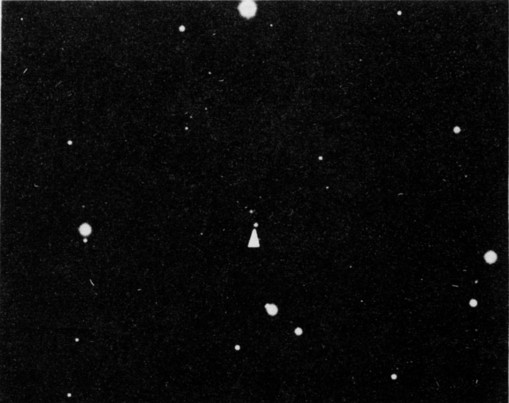
\includegraphics[scale=2.5 , keepaspectratio]{牧夫座中的3c295}
\caption{\footnotesize 最现代化的200英寸望远镜拍摄的最远天体——牧夫座中的3C295(用箭头标出)}
\end{figure}


\section{短的距离}
现在我们考虑一下小的距离。把一米分小是很容易的,把一米划分成一千个相等的间隔并没有多大困难。用相似的方法(利用一架好的显微镜),我们能够把1毫米分成一千等分,构成微米(一米的百万分之一)这样的尺度,但这要稍微困难一些。要继续分成更小的尺度则很困难,因为我们“看不见”一个比可见光波长(大约$ 5\times 10^{-7} $还要小的物体。

然而我们毋须停止在我们看得见的东西上,依靠电子显微镜,我们能用拍照方法来对更小的尺度(比方说一直到$ 10^{-8} $米)继续这个划分过程(图5-9)。
\begin{figure}[H]
\centering
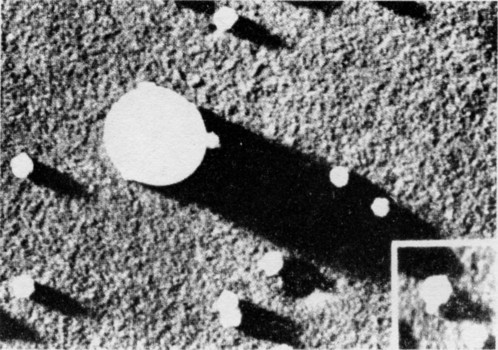
\includegraphics[scale=2.5 , keepaspectratio]{某些病毒分子的电子显微镜图}
\caption{\footnotesize 某些病毒分子的电子显微镜图。“大的”球是为定标用的,且已知其直径为$ 2\times 10^{-7} $米(2000 Å)}
\end{figure}
用间接的测量,即用一种显微镜规模的三角法,我们能对越来越小的尺度继续进行测量。首先我们从观察波长短的光(X射线)如何在间隔为已知的标记所组成的图样上被反射的情况,确定光振动的波长。然后从同样的光在一块晶体上所散射的图样,我们就能确定原子在晶体中的相对位置,所得结果与化学方法确定的原子间距离相符合。用这种方法我们发现原子的直径约为$10^{-10}$米。

典型的原子大小约为$10^{-10}$米,而原子核的大小为$10^{-15}$米,其间相差$10^5$倍!可见原子与原子核之间在物理大小上存在一个很大的“空隙”。对原子核的大小来说,用另一种测量方法比较方便。我们测量的是它的\uwave{表观面积}$\sigma$,称之为有效截面。如果要知道半径,则可从$\sigma=\pi r^2$求得,因为原子核是近似球形的。

核的截面可以这样来测量,使一束高能粒子通过某种材料的一块薄板,然后观察没有通过薄板的粒子数,这些高能粒子通常会穿过薄薄的电子云,而只有当它们碰上了质量集中的原子核时,才会被阻止或者被偏转。假设我们有一块$1$厘米厚的材料,其中大约有$10^8$个原子核。但原子核如此之小,以致一个核恰好位于另一个核的背后的机会是很小的。我们可以\uwave{设想},这种情况的一个高度放大的图像——沿着粒子束看去时——犹如图5-10所示。
\begin{figure}[H]
\centering
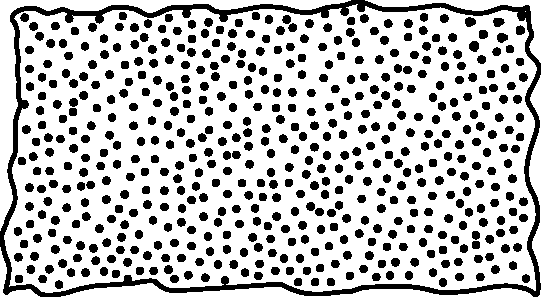
\includegraphics[scale=1 , keepaspectratio]{一块厚1厘米的碳设想的图像}
\caption{\footnotesize 在只观察核的时候,通过一块厚$1$厘米的碳所见到的那个设想的图像}
\end{figure}

一个很小的粒子在通过物质时能打在一个核上的几率,正好等于其中所有核的剖面所占的总面积除以这幅图上的总面积。假定我们知道在这块板的面积$A$中有$N$个原子(当然,每个原子只有一个核),那么被这些核所“覆盖”的面积和总面积之比就等于$N \sigma / A$。现在设粒子束中射到薄板的粒子数为$n_1$,从薄板另一边射出的粒子数为$n_2$。这样,\uwave{没有} 通过薄板的粒子数和射出的粒子数之比为$(n_1-n_2)/n_1$,它们应该正好等于被覆盖面积和总面积之比。于是从等式\footnote{只有当核所覆盖的面积是总面积的一个很小分数,即$(n_1-n_2)/n_1$远比1小时,这一等式才正确。否则我们必须对有些核将部分地为其前面的核所挡住这样的情况进行校正。}
\begin{equation*}
\pi r^2=\sigma=\frac{A}{N}\,
\frac{n_1-n_2}{n_1}.
\end{equation*}
就能获得核的半径。

从这样一种实验我们得出核的半径大约为$10^{-15}$米的一到六倍。$10^{-15}$米这个长度单位称为\uwave{费米},以纪念著名的物理学家费米(1901~1958)。

如果我们进到更小的距离,那么将会发生什么呢?能不能测量更小的距离?这样的问题现在还不可能回答。有人提出这种看法,认为迄今尚未解决的核力之谜,只有在对这样小的距离下的我们关于空间或测量的观念进行某些修正以后才能解开。

人们也许会想到,用某些自然长度来作为我们的长度单位——比如说地球的半径或者它的某一部分——倒是一个很好的意见。米之取作为单位只是出于这样的考虑,它被定义为地球半径的$(\pi/2)\times10^{-7}$倍。但是,用这种方法来规定长度单位,既不方便,也不很准确。很长时间以来国际上大家约定:一米的定义是保持在法国一个特殊实验室中的一根棒上两条刻线之间的距离。不久前人们认识到这个定义既未精确到足以使之有用,也不像人们所希望的那样稳定或普遍。近年来正在考虑采用一个新的定义,即选定一根光谱线,把大家一致同意的它的波长的(任意)倍数作为长度的单位。

\begin{fig}{一些时间举例}
\label{fig:一些时间举例}
\end{fig}

\begin{fig}{一些距离举例}
\label{fig:一些距离举例}
\end{fig}

\noindent\dotfill

距离测量和时间测量的结果有赖于观察者。两个作相互运动的观察者在测量看来似乎是同一个的事物时,将不会得到同样的距离和时间。距离和时间间隔随着测量时所用的坐标系(或“参考系”)不同而有不同的大小。我们将在后面的一章中详细地研究这个问题。

完全精密的距离测量或时间测量是为自然规律所不允许的。我们前面已经提到,在测量一个物体的位置时,误差至少要像
\begin{equation*}
\Delta x\geq\hbar/2\Delta p,
\end{equation*}
那样之大,其中$\hbar$是一个称为“普朗克常数”的很小的量,而$\Delta p$是我们在测量物体的位置时,对它的动量(质量乘以速度)的知识上的误差。我们也曾提到,位置测量的不确定性是与粒子的波动本质有关的。

空间和时间的相对性意味着时间的测量也有一个实际由
\begin{equation*}
\Delta t\geq\hbar/2\Delta E,
\end{equation*}
给出的最小误差,其中$\Delta E$是我们在测量一个过程的时间时,对它的能量的知识上的误差。如果我们要\uwave{更}精确地知道某个事件\uwave{何时}发生,那就只能对发生了什么知道得更少一点,因为我们对其所含能量的知识减少了。时间的不确定性也是与物质的波动本质有关的。



\chapter{几率}
\begin{quote}[J. C. 麦克斯韦]
我们这个世界的真正逻辑寓于几率的计算之中。
\end{quote}

\section{机会和可能性}
“机会”是日常生活中通常使用的一个词汇。无线电在播送明天的天气预报时可能会说:“明天下雨的机会是百分之六十。”你也许会说:“我能活上一百岁的机会是不大的。”科学家也使用机会这个词。一个地震学家可能会对这样的问题感兴趣:“明年在南加利福尼亚州发生某一级地震的机会有多大?”一个物理学家也许会提出这样的问题:“在下一个十秒钟内,某一特定盖革计数器将记录到20个计数的机会是多少?”一个政治家或国务活动家可能对下列问题感兴趣:“下一个十年内发生核战争的机会是多少?”同样,你也许会对从这一章中将学到一些的机会发生兴趣。

所谓\uwave{机会}指的是某种类似于猜测的事。为什么我们要猜测呢?希望作出判断而只掌握不完全的信息或不确定的知识时,我们就要进行猜测。我们要对这是些什么东西或者可能发生什么事情进行猜测。由于必须作出决定,我们常常要进行猜测。比如说,明天我是否要带上雨衣?我应设计一座能够防御哪种程度地震的新大厦?我是否要为自己建造一个放射性微粒掩蔽所?我是否要在国际谈判中改变自己的立场?我今天是否要去上课?

有时我们所以要进行猜测,是因为我们想用自己有限的知识来对某种情况说出\uwave{尽可能}多的东西。\textbf{事实上,任何一个判断本质上都是一种猜测。同样,任何物理理论都是一种猜测,其中有成功的,也有失败的}\footnote{这里只是简单提一下,实际上这句话蕴含了极深极丰富的哲学思想。}。概率论就是为进行较好猜测而产生的一种理论体系。应用几率的语言能使我们定量地谈论某些情况,而这些情况的变化可能很大,但确有某种一贯的平均行为。

让我们来研究向上抛掷硬币这件事。如果抛掷——以及硬币本身——都是“可靠”的,那么对任何一次特定的抛掷,我们无法预期能得到什么样的结果。然而我们可能会感到,在大量的抛掷中应该得到数目大致相等的正面和反面。我们说:“每次抛掷以正面落地的几率是0.5。”

我们只是为了对将来要做的那些观察而谈到几率的。\uwave{所谓在一次观察中将得到一个特定结果的“几率”,就是指我们在大量重复这个观察时对其中出现该特定结果的最可能分数的估计}。如果我们设想重复某种观察——比如看一下刚抛掷的硬币——$N$次,并且称$N_A$为\uwave{我们}对这些观察中最可能出现某一指定结果$A$——比如出现“正面”的数的\uwave{估计}。那么所谓观察到$A$的几率$P(A)$就是指:
\begin{equation}
\label{Eq:I:6:1}
P(A)=N_A/N.
\end{equation}

对我们这个定义,需要作几点注释。首先,只有当所发生的事件是某一\uwave{可重复}的观察的可能结果时,我们才能谈到发生某件事的几率。像“那所房子里出现一个幽灵的几率是多少?”这类问题有没有任何意义是不清楚的。

你可以争辩说,没有一种情况可以\uwave{不折不扣}地重复。这是对的。每一个不同的观察至少必须在不同的时间或者不同的地点进行。我们所能说的只是,对于我们想要达到的目的来说,凡是重复进行的观察应该看来似乎都是\uwave{等价的}。至少我们应当这样假定,每一次观察都在同样准备好的情况下进行,特别是在观察开始时都要带有同等程度的无知。(玩纸牌时,如果我们偷看一下对方的牌,那么我们对自己获胜的机会的估计就显然与偷看前不同!)

我们应当强调指出,式(6.1)中的$N$和$N_A$并\uwave{不}代表实际所作观察的次数。$N_A$是我们在$N$个\uwave{想像}的观察中\uwave{可能}得出结果$A$的观察的最佳\uwave{估计}。因此,几率有赖于我们的知识以及进行估计的能力。实际上有赖于我们的常识!幸运的是,常识对于许多事物都有一致程度的共同看法,所以不同的人将会作出同样的估计。然而,几率毋需是一些“绝对”的数字。既然它们与我们对事物的无知有关,那么如果我们所掌握的知识发生变化,它们也会变得不同。

你们也许已经注意到我们的几率定义中另一个相当“主观”的方面,我们把$N_A$说成是对最可能次数的一个估计……。可是这并不意味着我们\uwave{不折不扣}地期望能观察到$N_A$,而是期望能得到一个\uwave{靠近}$N_A$的数,而且数$N_A$比其邻近任何其他的数\uwave{更为可能}。比如说,我们抛掷一个硬币$30$次,那么我们可以预料,得到正面的数字不大可能正好是15,而很可能是某一靠近15的数,如12,13,14,15,16或17。然而,如果我们\uwave{必须}对之作出决择,那么我们就会决定,15次正面要比任何其他的数\uwave{更为可取}。我们将写成:P(正面)=0.5。

为什么我们选择15为一个比任何其他数更可取的数呢?我们一定会同自己以如下方式进行过争辩:如果在$N$次抛掷中得到正面的最可能次数为$N_H$,那么得到反面的最可能次数$N_T$就等于$N-N_H$。(这里我们作了这样的假定,即每次抛掷\uwave{不是}得到正面\uwave{便是}得到反面,不会得到“其他”结果! )但如果硬币是“可靠”的,它就既不偏向正面,也不偏向反面。除非有某些理由可以认为硬币(或者抛掷)是不可靠的,我们就必须认为正面与反面具有相等的可能性。所以必须使$N_T=N_H$。这样就得到$N_T=N_H=N/2$或者$P(H)=P(T)=0.5$。

我们可以把这一论证推广到任何一种情况;在这种情况下,可以观察到$m$个不同但又“相等”(即机会均等)的可能结果。如果通过观察能得到$m$个不同结果,而且又有理由相信,其中任何一个结果与别的任何结果同样可能,那么得到某一个\uwave{特定}结果$A$的几率就等于$P(A)=1/m$。

如果在一个不透明的盒子里有7个不同颜色的小球,我们“随便”(即不朝它看时)取出一个,那么得到某一种颜色的小球的几率是1/7。从已洗过的52张牌中“任意”抽出一张红桃10的几率是 掷骰子而得到两个一点的几率是
\begin{center}
\makebox[20
0pt]{\hrulefill}
\end{center}


从第五章中,我们用原子核的表观面积,或者称为截面来描写它的大小。这样做时,实际上我们就是在谈几率。当我们想一块薄的材料发射一个高能粒子时,它有一定机会直接穿过去,也有一定机会碰撞在一个原子核上。(既然原子核如此之小,以致我们无法看到,我们就不可能直接瞄准,而必须盲目射击。设在这块薄板中有n个原子,而每个原子的核具有截面积,那么被所有这些核所遮盖的总面积为n$\theta$



\section{起伏}
我们现在想利用有关几率的概念来比较详细地考虑一下这样的一个问题:“如果我把一个硬币抛掷N次,那么预期真正会得到多少次的正面?”然而在回答这个问题之前,让我们先来看一下在这样一个“实验”中确实会发生什么情况。图6-1表示N=30的这样一个实验在前三轮中所得到的结果,正面和反面的前后次序完全是按照它们得到时的次序排列的。第一轮得到11次正面;第二次也是11次;第三轮16次。在这三轮试验中,我们没有一回得到15次正面,是不是要对硬币发生怀疑呢?或者在这样一种游戏中,我们设想得到正面的最可能次数是15这一点错了呢?再做97轮实验,以便一共得到每回抛掷30次的实验100轮。实验的结果列在表6-1中

如果观察一下表6-1中所列出的各数,那么我们看到,大多数结果靠近15,而且位于12与18之间,如果我们为这些结果画一张分布图,那么就会对这些结果的细节有一个更好的理解。我们计算一下得到某一记录$k$的实验次数,并把这个数对每一个$k$作图,如图6-2所示,记录到15次正面的共13轮游戏,记录到14次正面的也是13轮。得到16的17次的,每一个都大于13轮,我们是否断定这里对正面有所偏袒?我们的最佳估计是否不够好,是不是我们现在不应该作出这个结论,即每轮30次抛掷的最可能记录实际上是16次正面,但是且慢,把所有各轮游戏加到一起,就总共抛掷了3000次,而获得正面的总数是1492次。可见出现正面的抛掷其比数是0.497,很接近而稍小于0.5。当然我们不应假定抛掷后得到正面的几率大于0.5!至于某特定的一组观察经常得到16次正面这个事实,是一种起伏现象,然而我们仍然预期最可能的正面数是15.

我们可以




\section{注释}
%\showendnotes
%这里空一行

\end{common-format}
\end{document}



